\documentclass[]{book}
\usepackage{lmodern}
\usepackage{amssymb,amsmath}
\usepackage{ifxetex,ifluatex}
\usepackage{fixltx2e} % provides \textsubscript
\ifnum 0\ifxetex 1\fi\ifluatex 1\fi=0 % if pdftex
  \usepackage[T1]{fontenc}
  \usepackage[utf8]{inputenc}
\else % if luatex or xelatex
  \ifxetex
    \usepackage{mathspec}
  \else
    \usepackage{fontspec}
  \fi
  \defaultfontfeatures{Ligatures=TeX,Scale=MatchLowercase}
\fi
% use upquote if available, for straight quotes in verbatim environments
\IfFileExists{upquote.sty}{\usepackage{upquote}}{}
% use microtype if available
\IfFileExists{microtype.sty}{%
\usepackage{microtype}
\UseMicrotypeSet[protrusion]{basicmath} % disable protrusion for tt fonts
}{}
\usepackage[margin=1in]{geometry}
\usepackage{hyperref}
\hypersetup{unicode=true,
            pdftitle={Course notes from MITx 14.310x Data Analysis for Social Scientists (EdX)},
            pdfauthor={James Solomon-Rounce},
            pdfborder={0 0 0},
            breaklinks=true}
\urlstyle{same}  % don't use monospace font for urls
\usepackage{natbib}
\bibliographystyle{apalike}
\usepackage{color}
\usepackage{fancyvrb}
\newcommand{\VerbBar}{|}
\newcommand{\VERB}{\Verb[commandchars=\\\{\}]}
\DefineVerbatimEnvironment{Highlighting}{Verbatim}{commandchars=\\\{\}}
% Add ',fontsize=\small' for more characters per line
\usepackage{framed}
\definecolor{shadecolor}{RGB}{248,248,248}
\newenvironment{Shaded}{\begin{snugshade}}{\end{snugshade}}
\newcommand{\KeywordTok}[1]{\textcolor[rgb]{0.13,0.29,0.53}{\textbf{#1}}}
\newcommand{\DataTypeTok}[1]{\textcolor[rgb]{0.13,0.29,0.53}{#1}}
\newcommand{\DecValTok}[1]{\textcolor[rgb]{0.00,0.00,0.81}{#1}}
\newcommand{\BaseNTok}[1]{\textcolor[rgb]{0.00,0.00,0.81}{#1}}
\newcommand{\FloatTok}[1]{\textcolor[rgb]{0.00,0.00,0.81}{#1}}
\newcommand{\ConstantTok}[1]{\textcolor[rgb]{0.00,0.00,0.00}{#1}}
\newcommand{\CharTok}[1]{\textcolor[rgb]{0.31,0.60,0.02}{#1}}
\newcommand{\SpecialCharTok}[1]{\textcolor[rgb]{0.00,0.00,0.00}{#1}}
\newcommand{\StringTok}[1]{\textcolor[rgb]{0.31,0.60,0.02}{#1}}
\newcommand{\VerbatimStringTok}[1]{\textcolor[rgb]{0.31,0.60,0.02}{#1}}
\newcommand{\SpecialStringTok}[1]{\textcolor[rgb]{0.31,0.60,0.02}{#1}}
\newcommand{\ImportTok}[1]{#1}
\newcommand{\CommentTok}[1]{\textcolor[rgb]{0.56,0.35,0.01}{\textit{#1}}}
\newcommand{\DocumentationTok}[1]{\textcolor[rgb]{0.56,0.35,0.01}{\textbf{\textit{#1}}}}
\newcommand{\AnnotationTok}[1]{\textcolor[rgb]{0.56,0.35,0.01}{\textbf{\textit{#1}}}}
\newcommand{\CommentVarTok}[1]{\textcolor[rgb]{0.56,0.35,0.01}{\textbf{\textit{#1}}}}
\newcommand{\OtherTok}[1]{\textcolor[rgb]{0.56,0.35,0.01}{#1}}
\newcommand{\FunctionTok}[1]{\textcolor[rgb]{0.00,0.00,0.00}{#1}}
\newcommand{\VariableTok}[1]{\textcolor[rgb]{0.00,0.00,0.00}{#1}}
\newcommand{\ControlFlowTok}[1]{\textcolor[rgb]{0.13,0.29,0.53}{\textbf{#1}}}
\newcommand{\OperatorTok}[1]{\textcolor[rgb]{0.81,0.36,0.00}{\textbf{#1}}}
\newcommand{\BuiltInTok}[1]{#1}
\newcommand{\ExtensionTok}[1]{#1}
\newcommand{\PreprocessorTok}[1]{\textcolor[rgb]{0.56,0.35,0.01}{\textit{#1}}}
\newcommand{\AttributeTok}[1]{\textcolor[rgb]{0.77,0.63,0.00}{#1}}
\newcommand{\RegionMarkerTok}[1]{#1}
\newcommand{\InformationTok}[1]{\textcolor[rgb]{0.56,0.35,0.01}{\textbf{\textit{#1}}}}
\newcommand{\WarningTok}[1]{\textcolor[rgb]{0.56,0.35,0.01}{\textbf{\textit{#1}}}}
\newcommand{\AlertTok}[1]{\textcolor[rgb]{0.94,0.16,0.16}{#1}}
\newcommand{\ErrorTok}[1]{\textcolor[rgb]{0.64,0.00,0.00}{\textbf{#1}}}
\newcommand{\NormalTok}[1]{#1}
\usepackage{longtable,booktabs}
\usepackage{graphicx,grffile}
\makeatletter
\def\maxwidth{\ifdim\Gin@nat@width>\linewidth\linewidth\else\Gin@nat@width\fi}
\def\maxheight{\ifdim\Gin@nat@height>\textheight\textheight\else\Gin@nat@height\fi}
\makeatother
% Scale images if necessary, so that they will not overflow the page
% margins by default, and it is still possible to overwrite the defaults
% using explicit options in \includegraphics[width, height, ...]{}
\setkeys{Gin}{width=\maxwidth,height=\maxheight,keepaspectratio}
\IfFileExists{parskip.sty}{%
\usepackage{parskip}
}{% else
\setlength{\parindent}{0pt}
\setlength{\parskip}{6pt plus 2pt minus 1pt}
}
\setlength{\emergencystretch}{3em}  % prevent overfull lines
\providecommand{\tightlist}{%
  \setlength{\itemsep}{0pt}\setlength{\parskip}{0pt}}
\setcounter{secnumdepth}{5}
% Redefines (sub)paragraphs to behave more like sections
\ifx\paragraph\undefined\else
\let\oldparagraph\paragraph
\renewcommand{\paragraph}[1]{\oldparagraph{#1}\mbox{}}
\fi
\ifx\subparagraph\undefined\else
\let\oldsubparagraph\subparagraph
\renewcommand{\subparagraph}[1]{\oldsubparagraph{#1}\mbox{}}
\fi

%%% Use protect on footnotes to avoid problems with footnotes in titles
\let\rmarkdownfootnote\footnote%
\def\footnote{\protect\rmarkdownfootnote}

%%% Change title format to be more compact
\usepackage{titling}

% Create subtitle command for use in maketitle
\newcommand{\subtitle}[1]{
  \posttitle{
    \begin{center}\large#1\end{center}
    }
}

\setlength{\droptitle}{-2em}

  \title{Course notes from MITx 14.310x Data Analysis for Social Scientists (EdX)}
    \pretitle{\vspace{\droptitle}\centering\huge}
  \posttitle{\par}
    \author{James Solomon-Rounce}
    \preauthor{\centering\large\emph}
  \postauthor{\par}
      \predate{\centering\large\emph}
  \postdate{\par}
    \date{2018-10-17}

\usepackage{booktabs}

\usepackage{amsthm}
\newtheorem{theorem}{Theorem}[chapter]
\newtheorem{lemma}{Lemma}[chapter]
\theoremstyle{definition}
\newtheorem{definition}{Definition}[chapter]
\newtheorem{corollary}{Corollary}[chapter]
\newtheorem{proposition}{Proposition}[chapter]
\theoremstyle{definition}
\newtheorem{example}{Example}[chapter]
\theoremstyle{definition}
\newtheorem{exercise}{Exercise}[chapter]
\theoremstyle{remark}
\newtheorem*{remark}{Remark}
\newtheorem*{solution}{Solution}
\begin{document}
\maketitle

{
\setcounter{tocdepth}{1}
\tableofcontents
}
\chapter*{Preface}\label{preface}
\addcontentsline{toc}{chapter}{Preface}

The following notes were taken by me for educational, non-commercial,
purposes. If you find the information useful, buy the material/take the
course.

Thank you to the original content providers. Additional ramblings are my
own.

\textbf{\emph{Core Resources}}

\begin{itemize}
\tightlist
\item
  \href{./files/14.310x_3T2018_Schedule.pdf}{Course Schedule}
\item
  \href{./files/14.310x_Grading_and_Homework_Policy__3T2018.pdf}{Grading
  and Homework Policy}
\item
  \href{./files/14310x_Honor_Code_and_Collaboration_Guidelines.pdf}{Honor
  Code and Collaboration Guide}
\item
  \href{./files/Derivation_of_OLS_Estimators.pdf}{Notes - OLS
  Derivation}
\item
  \href{./files/Matrix_Notation_etc.pdf}{Notes - Matrix Notation}
\item
  \href{https://www.rstudio.com/resources/cheatsheets/}{R Studio
  Cheatsheets}
\item
  \href{http://r4ds.had.co.nz/index.html}{R for Data Science Book}
\end{itemize}


\includegraphics[width=1\linewidth]{images/standing}

\chapter{Module 1: Introduction to the
Course}\label{module-1-introduction-to-the-course}

\begin{center}\rule{0.5\linewidth}{\linethickness}\end{center}

\textbf{Module Sections:}

\begin{itemize}
\tightlist
\item
  Welcome to the Course
\item
  Introduction to R
\item
  Introductory Lecture - Data is Beautiful, Insightful, Powerful,
  Deceitful
\item
  Finger Exercises
\item
  Module 1: Homework
\end{itemize}

Module Content:

\begin{itemize}
\tightlist
\item
  \href{./files/M1/Lecture_Slides_01.pdf}{Module 1 Slides}
\item
  \href{./files/M1/M1Paper.pdf}{Homework 1 Background Paper - The
  Persistent Effects Of Peru's Mining Mita}
\item
  \href{./files/M1/R_Instructions.pdf}{R Instructions}\\
\item
  \href{./files/M1/14_310x_Intro_to_R_.zip.pdf}{Intro to R Zip File}\\
\item
  \href{\%22./files/CitesforSara.csv\%22}{Citations Data for Homework 1}
\end{itemize}

\section{Introduction to R}\label{introduction-to-r}

First we setup the environment and install the course files

\begin{Shaded}
\begin{Highlighting}[]
\KeywordTok{library}\NormalTok{(swirl)}
\KeywordTok{install_course_zip}\NormalTok{(}\StringTok{"./files/M1/14_310x_Intro_to_R_.zip"}\NormalTok{,}\DataTypeTok{multi=}\OtherTok{FALSE}\NormalTok{)}
\KeywordTok{swirl}\NormalTok{()}
\end{Highlighting}
\end{Shaded}

IF z is a three number vector e.g.

\begin{Shaded}
\begin{Highlighting}[]
\NormalTok{z <-}\StringTok{ }\KeywordTok{c}\NormalTok{(}\FloatTok{1.1}\NormalTok{, }\DecValTok{9}\NormalTok{, }\FloatTok{3.14}\NormalTok{)}
\end{Highlighting}
\end{Shaded}

If we take the square root of z - 1 and assign it to a new variable
called my\_sqrt e.g.

\begin{Shaded}
\begin{Highlighting}[]
\NormalTok{my_sqrt <-}\StringTok{ }\KeywordTok{sqrt}\NormalTok{(z }\OperatorTok{-}\StringTok{ }\DecValTok{1}\NormalTok{)}
\end{Highlighting}
\end{Shaded}

The result is a vector of length three e.g.

\begin{Shaded}
\begin{Highlighting}[]
\NormalTok{my_sqrt}
\end{Highlighting}
\end{Shaded}

\begin{verbatim}
## [1] 0.3162278 2.8284271 1.4628739
\end{verbatim}

Next, if we create a new variable called my\_div that gets the value of
z divided by my\_sqrt.

\begin{Shaded}
\begin{Highlighting}[]
\NormalTok{my_div <-}\StringTok{ }\NormalTok{z }\OperatorTok{/}\StringTok{ }\NormalTok{my_sqrt}
\end{Highlighting}
\end{Shaded}

The first element of my\_div is equal to the first element of z divided
by the first element of my\_sqrt, and so on\ldots{}

\begin{Shaded}
\begin{Highlighting}[]
\NormalTok{my_div}
\end{Highlighting}
\end{Shaded}

\begin{verbatim}
## [1] 3.478505 3.181981 2.146460
\end{verbatim}

When given two vectors of the same length, R simply performs the
specified arithmetic operation (\texttt{+}, \texttt{-}, \texttt{*},
etc.) element-by-element. If the vectors are of different lengths, R
`recycles' the shorter vector until it is the same length as the longer
vector.

If the length of the shorter vector does not divide evenly into the
length of the longer vector, R will still apply the `recycling' method,
but will throw a warning.

\begin{Shaded}
\begin{Highlighting}[]
\KeywordTok{c}\NormalTok{(}\DecValTok{1}\NormalTok{, }\DecValTok{2}\NormalTok{, }\DecValTok{3}\NormalTok{, }\DecValTok{4}\NormalTok{) }\OperatorTok{+}\StringTok{ }\KeywordTok{c}\NormalTok{(}\DecValTok{0}\NormalTok{, }\DecValTok{10}\NormalTok{, }\DecValTok{100}\NormalTok{)}
\end{Highlighting}
\end{Shaded}

\begin{verbatim}
## Warning in c(1, 2, 3, 4) + c(0, 10, 100): longer object length is not a
## multiple of shorter object length
\end{verbatim}

\begin{verbatim}
## [1]   1  12 103   4
\end{verbatim}

\subsection{Module 1 Homework}\label{module-1-homework}

This is a sample of some of the homework answers. Some questions were
observational or required interpretation of maps for example, as such
these are not inluded here.

\begin{Shaded}
\begin{Highlighting}[]
\KeywordTok{library}\NormalTok{(tidyverse)}
\end{Highlighting}
\end{Shaded}

\begin{verbatim}
## -- Attaching packages ------------------ tidyverse 1.2.1 --
\end{verbatim}

\begin{verbatim}
## v ggplot2 3.0.0     v purrr   0.2.5
## v tibble  1.4.2     v dplyr   0.7.6
## v tidyr   0.8.1     v stringr 1.3.1
## v readr   1.1.1     v forcats 0.3.0
\end{verbatim}

\begin{verbatim}
## -- Conflicts --------------------- tidyverse_conflicts() --
## x dplyr::filter() masks stats::filter()
## x dplyr::lag()    masks stats::lag()
\end{verbatim}

\begin{Shaded}
\begin{Highlighting}[]
\NormalTok{papers <-}\StringTok{ }\KeywordTok{as_tibble}\NormalTok{(}\KeywordTok{read_csv}\NormalTok{(}\StringTok{"./files/M1/CitesforSara.csv"}\NormalTok{))}
\end{Highlighting}
\end{Shaded}

\begin{verbatim}
## Parsed with column specification:
## cols(
##   .default = col_integer(),
##   journal = col_character(),
##   title = col_character(),
##   au1 = col_character(),
##   au2 = col_character(),
##   au3 = col_character(),
##   past5 = col_double(),
##   aflpn90 = col_double(),
##   aulpn90 = col_double(),
##   aulpn80 = col_double(),
##   aulpn70 = col_double(),
##   lcites = col_double()
## )
\end{verbatim}

\begin{verbatim}
## See spec(...) for full column specifications.
\end{verbatim}

Q. 19 Let's take a look at some of the most popular papers. Using the
filter() method, how many records exist where there are greater than or
equal to 100 citations?

\begin{Shaded}
\begin{Highlighting}[]
\CommentTok{#First lets look at our data}
\KeywordTok{head}\NormalTok{(papers)}
\end{Highlighting}
\end{Shaded}

\begin{verbatim}
## # A tibble: 6 x 22
##   journal  year cites title au1   au2   au3   female1 female2 female3  page
##   <chr>   <int> <int> <chr> <chr> <chr> <chr>   <int>   <int>   <int> <int>
## 1 Americ~  1993    31 Jeux~ Kanb~ Keen~ <NA>        0       0      NA    16
## 2 Americ~  1993     4 Chan~ Jame~ <NA>  <NA>        0      NA      NA    22
## 3 Americ~  1993    28 Fact~ Bert~ <NA>  <NA>        0      NA      NA    15
## 4 Americ~  1993    10 Stra~ Garf~ Oh,-~ <NA>        1       0      NA    19
## 5 Americ~  1993     5 Will~ Coat~ Lour~ <NA>        0       0      NA    21
## 6 Americ~  1993    21 Merg~ Kim,~ Sing~ <NA>        0       0      NA    21
## # ... with 11 more variables: order <int>, nauthor <int>, past5 <dbl>,
## #   aflpn90 <dbl>, spage <int>, field <int>, subfld <int>, aulpn90 <dbl>,
## #   aulpn80 <dbl>, aulpn70 <dbl>, lcites <dbl>
\end{verbatim}

\begin{Shaded}
\begin{Highlighting}[]
\KeywordTok{arrange}\NormalTok{(papers,}\KeywordTok{desc}\NormalTok{(cites), title)}
\end{Highlighting}
\end{Shaded}

\begin{verbatim}
## # A tibble: 4,182 x 22
##    journal  year cites title au1   au2   au3   female1 female2 female3
##    <chr>   <int> <int> <chr> <chr> <chr> <chr>   <int>   <int>   <int>
##  1 Econom~  1980  2251 A He~ Whit~ <NA>  <NA>        0      NA      NA
##  2 Econom~  1979  2227 Pros~ Kahn~ Tver~ <NA>        0       0      NA
##  3 Econom~  1987  2164 Co-i~ Engl~ Gran~ <NA>        0       0      NA
##  4 Econom~  1979  1602 Samp~ Heck~ <NA>  <NA>        0      NA      NA
##  5 Econom~  1978  1217 Spec~ Haus~ <NA>  <NA>        0      NA      NA
##  6 Econom~  1982  1077 Auto~ Engl~ <NA>  <NA>        0      NA      NA
##  7 Econom~  1981  1031 Like~ Dick~ Full~ <NA>        0       0      NA
##  8 Econom~  1982   983 Larg~ Hans~ <NA>  <NA>        0      NA      NA
##  9 Econom~  1980   864 Macr~ Sims~ <NA>  <NA>        0      NA      NA
## 10 Econom~  1982   563 Time~ Kydl~ Pres~ <NA>        0       0      NA
## # ... with 4,172 more rows, and 12 more variables: page <int>,
## #   order <int>, nauthor <int>, past5 <dbl>, aflpn90 <dbl>, spage <int>,
## #   field <int>, subfld <int>, aulpn90 <dbl>, aulpn80 <dbl>,
## #   aulpn70 <dbl>, lcites <dbl>
\end{verbatim}

\begin{Shaded}
\begin{Highlighting}[]
\NormalTok{papers }\OperatorTok
\StringTok{  }\KeywordTok{filter}\NormalTok{(cites }\OperatorTok{>=}\StringTok{ }\DecValTok{100}\NormalTok{) }
\end{Highlighting}
\end{Shaded}

\begin{verbatim}
## # A tibble: 205 x 22
##    journal  year cites title au1   au2   au3   female1 female2 female3
##    <chr>   <int> <int> <chr> <chr> <chr> <chr>   <int>   <int>   <int>
##  1 Americ~  1994   117 Is I~ Pers~ Tabe~ <NA>        0       0      NA
##  2 Econom~  1971   149 Furt~ Nerl~ <NA>  <NA>        0      NA      NA
##  3 Econom~  1971   170 The ~ Madd~ <NA>  <NA>       NA      NA      NA
##  4 Econom~  1971   155 Inve~ Luca~ Pres~ <NA>        0       0      NA
##  5 Econom~  1971   139 Some~ Crag~ <NA>  <NA>        0      NA      NA
##  6 Econom~  1971   108 Iden~ Roth~ <NA>  <NA>        0      NA      NA
##  7 Econom~  1972   164 Meth~ Fair~ Jaff~ <NA>        0       0      NA
##  8 Econom~  1972   150 Exis~ Radn~ <NA>  <NA>        0      NA      NA
##  9 Econom~  1973   361 Mani~ Gibb~ <NA>  <NA>        0      NA      NA
## 10 Econom~  1973   107 On a~ Kram~ <NA>  <NA>        0      NA      NA
## # ... with 195 more rows, and 12 more variables: page <int>, order <int>,
## #   nauthor <int>, past5 <dbl>, aflpn90 <dbl>, spage <int>, field <int>,
## #   subfld <int>, aulpn90 <dbl>, aulpn80 <dbl>, aulpn70 <dbl>,
## #   lcites <dbl>
\end{verbatim}

Q.20 Use the group\_by() function to group papers by journal. How many
total citations exist for the journal ``Econometrica''?

\begin{Shaded}
\begin{Highlighting}[]
\NormalTok{papers }\OperatorTok
\StringTok{  }\KeywordTok{group_by}\NormalTok{(journal) }\OperatorTok
\StringTok{  }\KeywordTok{summarise}\NormalTok{(}\KeywordTok{sum}\NormalTok{(cites))}
\end{Highlighting}
\end{Shaded}

\begin{verbatim}
## # A tibble: 7 x 2
##   journal                            `sum(cites)`
##   <chr>                                     <int>
## 1 American-Economic-Review                   3738
## 2 Econometrica                              75789
## 3 Journal-of-Political-Economy               3398
## 4 Quarterly-Journal-of-Economics             8844
## 5 Review-of-Economic-Studies                21937
## 6 Review-of-Economics-and-Statistics         8473
## 7 <NA>                                         14
\end{verbatim}

\begin{Shaded}
\begin{Highlighting}[]
\CommentTok{#or}

\KeywordTok{summarize}\NormalTok{(group_by}
\NormalTok{          (papers, journal), }
          \DataTypeTok{SumOfCites =} \KeywordTok{sum}\NormalTok{(cites))}
\end{Highlighting}
\end{Shaded}

\begin{verbatim}
## # A tibble: 7 x 2
##   journal                            SumOfCites
##   <chr>                                   <int>
## 1 American-Economic-Review                 3738
## 2 Econometrica                            75789
## 3 Journal-of-Political-Economy             3398
## 4 Quarterly-Journal-of-Economics           8844
## 5 Review-of-Economic-Studies              21937
## 6 Review-of-Economics-and-Statistics       8473
## 7 <NA>                                       14
\end{verbatim}

Q.21 How many distinct primary authors (au1) exist in this dataset?

\begin{Shaded}
\begin{Highlighting}[]
\NormalTok{papers }\OperatorTok
\StringTok{  }\KeywordTok{summarise}\NormalTok{(}\KeywordTok{n_distinct}\NormalTok{(au1))}
\end{Highlighting}
\end{Shaded}

\begin{verbatim}
## # A tibble: 1 x 1
##   `n_distinct(au1)`
##               <int>
## 1              2332
\end{verbatim}

\begin{Shaded}
\begin{Highlighting}[]
\CommentTok{#or}

\KeywordTok{n_distinct}\NormalTok{(papers}\OperatorTok{$}\NormalTok{au1)}
\end{Highlighting}
\end{Shaded}

\begin{verbatim}
## [1] 2332
\end{verbatim}

\chapter{Module 2: Fundamentals of Probability, Random Variables, Joint
Distributions + Collecting
Data}\label{module-2-fundamentals-of-probability-random-variables-joint-distributions-collecting-data}

\begin{center}\rule{0.5\linewidth}{\linethickness}\end{center}

\textbf{Module Sections:}

\begin{itemize}
\tightlist
\item
  Fundamentals of Probability
\item
  Random Variables, Distributions, and Joint Distributions
\item
  Gathering and Collecting Data
\item
  Module 2: Homework
\end{itemize}

Module Content:

\begin{itemize}
\tightlist
\item
  \href{./files/M1/Lecture_Slides_02.pdf}{Section 2 Slides -
  Fundamentals of Probability}
\item
  \href{./files/M1/Lecture_Slides_03.pdf}{Section 3 Slides - Random
  Variables, Distributions and Joint Distributions}
\item
  \href{./files/M1/Gathering_Data.pdf}{Section 4 Slides - Gathering and
  Collecting Data}
\end{itemize}

\section{Fundamentals of Probability}\label{fundamentals-of-probability}

\subsection{Set Theory}\label{set-theory}

\begin{itemize}
\item
  A \emph{sample space} is collection of all possible outcomes
\item
  An \emph{event} is any collection of outcomes - could be one, all or
  none
\item
  If the outcome is a member of an event, the event is said to have
  \emph{occured}
\item
  Event B is said to be \emph{contained} by A, if all outcomes in B also
  are in A
\item
  This is the basis of set theory and used widely in probability,
  although there are some differences between set and probability theory
\item
  If there is no symbol, then this usually means intersection AB in
  probability - in set theory we would write an inverted U e.g.
  \(A \cap B\)
\item
  A and B are mutually exclusive (disjoint in set theory) if they have
  no outcomes in common
\item
  A and B are exhaustive (complimentary in set theory) if their union is
  S (the entire sample space)
\item
  A and B are both mutually exclusive and exhaustive, their union is
  equal to the sample space but they have no events in common - they are
  a partition of the sample space
\end{itemize}

\subsection{Defining Probability}\label{defining-probability}

We assign every event a number P(A) which is the prob. the event will
occur

1 We require that the probability is greater than one for all events in
the sample space - P(A) \textgreater{}= 0 for all A c S 2 The entire
sample space must be equal to one - P(S) = 1 3 For any sequence of
disjoint sets, the prob. of the union of that sequence is equal to the
sum of the probabilities of those events - A\textsubscript{1},
A\textsubscript{2}, \ldots{} , is P(V\textsubscript{i}) =
\(\sum_{i} P(A_i)\)

So we have a sample space, and if it satisfies these three properties,
then we call it a probability. Sometimes this is referred to as a
probability function or a probability distribution, but there is no
standard terminology for all probability theory. Set theory helps to
prove aspects of probability mathematically, for the purposes on this
course, we just need to know what some useful facts are.

\begin{itemize}
\tightlist
\item
  P(A\textsuperscript{c}) = 1 - P(A) =
\end{itemize}

The probability of A compliment, which is the event that contains all of
the outcomes that are not in the event A, the probability of A
compliment is just equal to 1 minus the probability of A. This is useful
if the probability of A comliment (P(A\textsuperscript{c})) is difficult
to compute, where as the probability of A might be very easy to compute.

\begin{itemize}
\tightlist
\item
  \(P (\emptyset)\) =
\end{itemize}

The probability of the empty set is zero.

\begin{itemize}
\tightlist
\item
  If A \textsubscript{c} B then P(A) \textless{}= P(B) =
\end{itemize}

If A is contained in B then the probability of A is less than or equal
to the probability of B

\begin{itemize}
\tightlist
\item
  For all A, 0 \textless{}= P(A) \textless{}= 1 =
\end{itemize}

For any events, the probability of that event is between 0 and 1.

\begin{itemize}
\tightlist
\item
  P(AUB) = P(A) + P(B) - P(AB) =
\end{itemize}

Probability of A union B is just equal to the sum of the probabilities
of those two events minus the probability of the their intersection.

\begin{itemize}
\tightlist
\item
  P(AB\textsuperscript{c}) = P (A) - P(AB) =
\end{itemize}

The probability of A times B complement is equal to the probability of A
minus the probability of the intersection.

\subsection{An example}\label{an-example}

Suppose you have a finite sample space. Let the function n(.) give the
number of elements in a set.

Then define P(A) = n(A)/n(S). This is called a simple sample space, and
it is a probability - we count the number of outcomes and divide by the
number of possible outcomes in the sample space.

We can check that it satisfies the three axioms to ensure it is a
probability:

\begin{enumerate}
\def\labelenumi{\arabic{enumi}.}
\tightlist
\item
  P(A) will always be non-negative because it's a count
\item
  P(S) will equal 1, by definition
\item
  P(AUB) = n(AUB)/n(S) = n(A)/n(S) + n(B)/n(S) = P(A) +P(B).
\end{enumerate}

If you can put your experiment in to this sample space where each
outcome is equally likely, we just need to count to calculate
probabilities of events. So for example, if you want to know how likely
it is you will roll a specific number, say 6, on two dice, we calculate
all the different ways that six occurs then divide this by all possible
outcomes (sample space) - = 5 / 36 = or 13.9\%

\subsection{Another example}\label{another-example}

If the state of Massachusetts issues 6-character license plates, using
one of 26 letters and 10 digits randomly for each character, what is the
probability that I will receive an all digit license plate?

n(S) = 36 (26 + 10) possibilities for each of 6 characters =
36\textsuperscript{6} = 2.176b n(A) = 10 possibilities (for digits only)
for each of 6 characters = 10\textsuperscript{6} = 1m so P(A) = .0005

This is \emph{sampling with replacement}

\emph{What if Massachusetts does not reuse a letter or digit?}

Now, in the sample space, there are 36 possibilities (26 + 10) for the
1st character, 35 left for the 2nd, and so on.

n(S) = 36x35x34x33x32x31 = 36!/30! = 1.402b

Similarly, in the event, there are 10 possibilities for the 1st
character, 9 left for the 2nd, and so on.

n(A) = 10x9x8x7x6x5 = 10!/4! = 151k

so P(A) = 1.402b / 151k = .0001

This is \emph{sampling without replacement}

\subsection{Ordered and Unordered
Arrangements}\label{ordered-and-unordered-arrangements}

In the examples so far, we have used a series of counting rules -
combinatorics i.e.~combinations of objects belonging to a finite set in
accordance with certain constraints.

\begin{enumerate}
\def\labelenumi{\arabic{enumi}.}
\item
  If an experiment has two parts, first one having m possibilities and,
  regardless of the outcome in the first part, the second one having n
  possibilities, then the experiment has m * n possible outcomes - this
  is what we do intuitively
\item
  Any ordered arrangement of objects is called a \emph{permutation}. The
  number of different permutations of N objects is N! The number of
  different permutations of n objects taken from N objects is N!/(N-n)!
  This is the case in the license plate example previously given
\item
  Any unordered arrangement of objects is called a \emph{combination}.
  The number of different combinations of n objects taken from N objects
  is N!/\{(N-n)!n!\}. We typically denote this \(\binom{N}{n}\) - N (big
  objects) choose n (combinations). This is where the order of objects
  doesn't matter i.e.~different orderings don't matter - we take out the
  ordering
\end{enumerate}

So if we had 9 people who each wanted to shake hands, if order doesn't
matter then it is a combination and we take 9 and choose 2 so it
becomes:

9! / \{(9-2)! * 2!\} = 9! / \{7! * 2!\} = 362,880 / \{5,040 * 2\} =
362,880 / 10,080 = 36 combinations

Note, if order did matter and we used the permutations formula the total
would be twice as many

\subsection{Office Arrangements and Pizza
Toppings}\label{office-arrangements-and-pizza-toppings}

Q: If there are six vegetarian pizza toppings and five non-veg, if I
randomly choose two from a hat containing all items, what is the
probability that I end up with a pizza that has one veg and one non-veg
topping?

A:

First we need to count the number of possabilities in the sample space
e.g. \{(V1, V2), (V1, V3), (V1, V4), (V1, N1) \ldots{}\} n(S) =
\(\binom{11}{2}\) = 55 - All outcomes are equally likely

Now we need to define our outcome n(A) = there are A = \{(V1, N1), (V1,
N2), (V2, N1) \ldots{} \} n(A) = 6 * 5 = 30

So the probability is N(A) / n(S) = 30 / 55 = 0.55

In general, I could have chose n toppings and asked what is the
probability that my pizza had n1 vegetarian toppings and n2
non-vegetarian toppings. There would, then, be \(\binom{6}{n_1}\)
possibilities for the veg toppings and \(\binom{5}{n_2}\)for the non-veg
toppings. In other words,

\[P(n_1 veg, n_2  non-veg)=  \binom{6}{n_1} \binom{5}{n_2} \\ \binom{11}{n}\]
This is the basis of the hypergeometric distribution.

\subsection{Independence and Basketball
Example}\label{independence-and-basketball-example}

We call probabilistic events stochastic events. One of the most
fundamental relationships between stochastic events is independence.

\begin{itemize}
\tightlist
\item
  Events A and B are independent if P(AB) = P(A) P(B)
\end{itemize}

That is to say, events A and B are independent if the probability of
their intersection is equal to the product of their probabilities.

\begin{itemize}
\tightlist
\item
  independent events is that knowing one event occurred doesn't give you
  any information about whether the other occurred.
\end{itemize}

This is best represented with an example. If you toss one die, once.
Consider the event, A, that you roll a number less than 5, and the
event, B, that you roll an even number. Are these events independent?

You might consider how could they be, as they rely on the same roll of a
die?

If we use the previous example for independence, we check:

\begin{enumerate}
\def\labelenumi{\arabic{enumi}.}
\item
  Probability of event A is P(A) = 2/3
\item
  Probability of event B is P(B) = 1/2
\item
  Probability of their intersection is P(AB) = 1/3 which is the same as
  P(A) P(B)
\end{enumerate}

So yes, it does satisfy the definition of independence. AB is rolling an
even number less than 5 (e.g.~2 or 4) and P(A)P(B) = P(AB)

\textbf{So knowing one event occurred doesn't give you any information
about whether an other occured}

In another example, if we had a bag of ten poker chips numbered 1 to 10,
with 3 different colours - \(\color{red}{\text{Red(1,2,3,4,5)}}\),
\(\color{blue}{\text{Blue(6,7)}}\) or
\(\color{green}{\text{Green(8,9,10)}}\)

If choosing a poker chip, A that it is blue, and B that it is even,
independent?

\begin{enumerate}
\def\labelenumi{\arabic{enumi}.}
\item
  Probability of event A is P(A) = 2/10 (.2)
\item
  Probability of event B is P(B) = 5/10 (.5)
\item
  Probability of their intersection is P(AB) = 1/10 (or .1) which is the
  same as P(A) P(B)
\end{enumerate}

So yes they are independent, knowing one (that it is blue) does not give
you any information about an other event (it is even).

Note that mutually exclusivity (disjoint events) and independence are
not the same. Mutually exclusive events are not independent, and
independent events cannot be mutually exclusive. Events are mutually
exclusive if P (A and B) = 0.

So our independent events - blue and even - are not mutually exclusive,
they can occur at the same time. Put another way, because events can't
happen at the same time (disjoint or mutually exclusive), they can't be
independent.

So if we take two mutually exclusive events - say the probability of a
poker chip being both green (A) and blue (B) - we can check for the
three parts of independence as:

\begin{enumerate}
\def\labelenumi{\arabic{enumi}.}
\item
  Probability of event A is P(A) = 3/10 (.3)
\item
  Probability of event B is P(B) = 2/10 (.2)
\item
  Probability of their intersection is P(AB) = 0 which is not the same
  as P(A) P(B) (which is 0.06)
\end{enumerate}

As P (AB) = 0 i.e.~they are mutually exclusive they are dependent -
knowing one i.e.~the chip blue DOES give you information about whether
the other event occured - you know it is not green, so the probability
of being green goes from 30\% before being told, to 0\% after being told
it is blue.

\textbf{When events are mutually exclusive, when you know one thing is
true the likelihood of the otehr being true becomes zero}

For more than two events, we define independence the same way - the
events are independent if the probability of their intersection is equal
to the product of their probabilities.

\subsection{Conditional Probability}\label{conditional-probability}

What if knowing one event has occured tells us something about the
probability that another event occured? How can we `update' our
knowledge in the event that the first event has occured?

The probability of A conditional on B is denoted as P(A\textbar{}B). So
the probability of A conditional on B, P(A\textbar{}B), is P(AB)/ P(B),
assuming P(B) \textgreater{} 0. We don't condition on an event if the
probability of an event is 0\%.

So in effect, by knowing one event has occured, it changes or re-defines
our numerator for event B AND it is changing or re-defining our
denominator - the part of the sample space which is now relevant - of
event B.

There is a relationship between indepdence and conditional probability.
Suppose A and B are independent and P(B) \textgreater{} 0. Then,

P(A\textbar{}B) = P(AB)/P(B) = P(A)P(B) (as they are indepdent this is
the same as P(AB)) / P(B) = P(A) (we cancel out P(B) from the previous)

or simply

P(A\textbar{}B) = P(AB)/P(B) = P(A)P(B)/P(B) = P(A)

\subsection{Conditional Probability in American Presidential
Politics}\label{conditional-probability-in-american-presidential-politics}

If candidates for Republican nomination had the following probabilities
- these might be obtained from looking at betting markets

Trump P(A\textsubscript{1}) = .4\\
Cruz P(A\textsubscript{2}) = .3\\
Rubio P(A\textsubscript{3}) = .2\\
Carson P(A\textsubscript{4}) = .1

How can we compute the probability of a Republican win for the
presidency or P(W) i.e.~the general election?

Conditional on winning the nomination, the candidates have following
probabilities of winning the general election:

Trump P(W\textbar{}A\textsubscript{1}) = .25\\
Cruz P(W\textbar{}A\textsubscript{2}) = .2\\
Rubio P(W\textbar{}A\textsubscript{3}) = .6\\
Carson P(W\textbar{}A\textsubscript{4}) = .4

The probability of a Republic win is equal to the probability of the
intersection between a Republican win and the sample space.

The sample space is the union between the four events A1 through A4. A1
through A4 are mutually exclusive and exhaustive events and therefore
form a partition.

In terms of notation, we therefore have:

P(W) = P(WS)

= P(W(A\textsubscript{1} U A\textsubscript{2} U A\textsubscript{3} U
A\textsubscript{4})) because A1-A4 are mutually exclusive and exhaustive
sets, a partition\\
= P(WA\textsubscript{1} U WA\textsubscript{2} U WA\textsubscript{3} U
WA\textsubscript{4})\\
= P(WA\textsubscript{1}) + P(WA\textsubscript{2}) +
P(WA\textsubscript{3}) + P(WA\textsubscript{4})\\
= P(W\textbar{}A\textsubscript{1})P(A\textsubscript{1}) +
P(W\textbar{}A\textsubscript{2})P(A\textsubscript{2}) +
P(W\textbar{}A\textsubscript{3})P(A\textsubscript{3}) +
P(W\textbar{}A\textsubscript{4})P(A\textsubscript{4})

So P(W) = .4x.25 + .3x.2 + .2x.6 + .1x.4 = .32

\subsection{Bayes' Theorem}\label{bayes-theorem}

So far, we have seen that the probability of the intersection between A
and B is equal to the Probability of B conditional on A times the
probability of A:

\begin{itemize}
\tightlist
\item
  P(AB) = P(B\textbar{}A)P(A) = P(A\textbar{}B)P(B)
\item
  provided P(A) \textgreater{} 0 and P(B) \textgreater{} 0 i.e.~both A
  and B have positive probabilities
\item
  so we can write P(A\textbar{}B) = P(B\textbar{}A)P(A)/P(B)
\end{itemize}

We also saw a slightly more complicated version of this, where the
probability of B is the probability of B conditional on A times the
probability of A, plus the probability of B conditional on A complement
times the probability of A complement (note we saw this, albeit with
more compliments, when looking at the Conditional Probability in
American Presidential Politics section)

\begin{itemize}
\tightlist
\item
  P(B) = P(B\textbar{}A)P(A) + P(B\textbar{}Ac)P(Ac)
\item
  P(A\textbar{}B) = P(B\textbar{}A)P(A)/\{P(B\textbar{}A)P(A) +
  P(B\textbar{}Ac)P(Ac)\}
\end{itemize}

C is compliment, and we can do this since A and Ac are partitions of the
sample space S.

A pregnant woman lives in an area where the Zika virus is fairly rare -
1 in 1000 people have it. Still, she's concerned, so she gets tested.
There is a good but not perfect test for the virus---it gives a positive
reading with probability .99 if the person has the virus and a positive
reading with probability .05 if the person does not. Her reading is
positive. How concerned should we be?

P(Z) = .001 (unconditional probability of having Zika) P(Zc) = .999 (999
people don't have it) P(+\textbar{}Z) = .99 (probability of having a
positive test result, conditional on having the zika virus - there is a
1\% change of a false negative) P(+\textbar{}Zc) = .05 (probability of
having a positive result if you don't have the virus is 5\% - false
positive rate) P(Z\textbar{}+) =
P(+\textbar{}Z)P(Z)/\{P(+\textbar{}Z)P(Z) + P(+\textbar{}Zc)P(Zc)\} -
Bayes theorem = .019 - less than 2\% probability

So the introduction of our new data results in us updating our
probability based on the imperfect test, but it doesn't get updated by
much as it still possible it's wrong and the prevelance rate of the zika
virus is rare.

\emph{Example 2}

Assume that the probability of having a rare condition is 1\%. It is
possible to test for the condition, but the test is imperfect. If you
have the condition, there is an 85\% chance that you will test positive.
If you do not have the condition, there is a 5\% chance that you will
test positive. Call the condition C, so that P(C) = 0.01, and call a
positive test t+, so that p(t+\textbar{}C) = 0.85.

What is the probability p(t+) that you test positive for the condition?

So the Probability of having the condition is P(C) 0.01 *
P(t+\textbar{}C) = .85 which is the probability at a test you will test
positive = 0.0085 + P(Cc) * P(t+\textbar{}Cc) = 0.99 * 0.05 = 0.0495 =
0.058

Suppose that you tested positive for the condition. What is the
probability that you truly have the underlying condition?

P(C) = .01 (unconditional probability of having condition) P(Cc) = .99
(99 people don't have it) P(t+\textbar{}C) = .85 (probability of having
a positive test result, conditional on having the condition)
P(t+\textbar{}Cc) = .05 (probability of having a positive result if you
don't have the virus is 5\% - false positive rate) P(C\textbar{}+) =
P(t+\textbar{}C)P(C)/\{P(t+\textbar{}C)P(C) + P(t+\textbar{}Cc)P(Cc)\} -
Bayes theorem = 0.0085 / \{0.0085 + 0.0495\} = .15 - around than 15\%
probability

Suppose that a new test is developed that is more accurate. Now, the
probability of testing positive if you have the condition is 94\%, and
the chance of testing positive if you do not have the condition is only
4\%. Now, what is the probability p(t+) that you test positive for the
condition?

So the Probability of having the condition is P(C) 0.01 *
P(t+\textbar{}C) = .94 which is the probability at a test you will test
positive = 0.0094 + P(Cc) * P(t+\textbar{}Cc) = 0.99 * 0.04 = 0.0396 =
0.049

Suppose that you tested positive for the condition. What is the
probability that you truly have the underlying condition?

P(C) = .01 (unconditional probability of having condition)\\
P(Cc) = .99 (99 people don't have it)\\
P(t+\textbar{}C) = .94 (probability of having a positive test result,
conditional on having the condition)\\
P(t+\textbar{}Cc) = .04 (probability of having a positive result if you
don't have the virus is 5\% - false positive rate)\\
P(C\textbar{}+) = P(t+\textbar{}C)P(C)/\{P(t+\textbar{}C)P(C) +
P(t+\textbar{}Cc)P(Cc)\} - Bayes theorem\\
= 0.0094 / \{0.0094 + 0.0396\}\\
= .19 - around than 15\% probability

Suppose that there is an 80\% chance you will be invited to a dinner
party on a Friday or Saturday evening. In contrast, there is only a 50\%
chance that you will be invited to a dinner party on one of the other
nights of the week. Suppose that you know that you've been invited to a
dinner party tonight, but have forgotten which day of the week it is.
Once you know that you've been invited to a dinner party, what is the
chance that it is either Friday or Saturday? (Please round your answer
to 2 decimal places. For example, if the correct answer is 0.6724,
please input 0.67.)

Hint: Using the notation of Zika question, Let Z:= \{ Fri, Sat\} and
Z\^{}c = \{ M,T,W,Th,Sun\}. Let ``+'' denote invitation. You are given
Pr(``+''\textbar{} Z) = 0.8 and Pr(``+''\textbar{} Z\^{}c) = 0.5. We
want to compute Pr( Z \textbar{} ``+'')

P(Z) = .286 (unconditional probability of it being Friday or Saturday)\\
P(Zc) = .714 (the other 5 days of the week)\\
P(+\textbar{}Z) = .8\\
P(+\textbar{}Zc) = .5\\
P(Z\textbar{}+) = P(+\textbar{}Z)P(Z)/\{P(+\textbar{}Z)P(Z) +
P(+\textbar{}Zc)P(Zc)\} - Bayes theorem\\
= .389 - around 40\% probability

\section{Random Variables, Distributions and Joint
Distributions}\label{random-variables-distributions-and-joint-distributions}

A \emph{random variable} is a real-valued function whose domain is the
sample space - it goes from the sample space to the real line.

A probability goes from the set of all subsets of the sample space in to
the unit interval e.g. {[}0,1{]} between zero and 1

A random variable goes from the sample space to the real line and it has
some numerial charecteristics of the sample space we are interested in.

The probability that something exists induces a distribution of the
random variable, they are not the same.

There are two types of random variable:

\begin{itemize}
\tightlist
\item
  Discrete - one that can take on only a - finite or infinite -
  countably number of values
\item
  Continous - a random variable that can take on any value in some
  interval, bounded or unbounded, of the real line
\end{itemize}

Discrete random variables can be approximated using a continous random
variable, so we typically just use continous. Most of the example we
have seen so far in this section have dealt with discreet random
variables.

\subsection{Probability Functions of Random
Variables}\label{probability-functions-of-random-variables}

For discrete random variables, we often start with a verbal description,
calculate probabilities for each value of the random variable, and then
write down a function or draw a graph describing those probabilities for
different values of the random variable. This is called a probability
function (PF). We saw one of these before in the hypogeometric and
binomial, when looking at the pizza toppings.

Note that:

\begin{itemize}
\tightlist
\item
  The term probability density function is used to draw attention to the
  fact that we are discussing a continuous random variable.\\
\item
  The term probability mass function is used to draw attention to the
  fact that we are discussing a discrete random variable.\\
\item
  The term probability function - or sometimes just the term
  ``distribution'' - is used when we are speaking in more general terms,
  when we're discussing both ``flavors'' of probability function or the
  distinction between the two types of probability functions/random
  variables doesn't matter.
\end{itemize}

Hypergeometric (pizza topping) random variable:

1 Verbal description - Let X be the number of vegetarian toppings I get
on my pizza if I draw the Area Four toppings randomly (without
replacement)

2 Calculation - We can calculate the probability that X = 0, 1, 2, and
so forth, up to the maximum of 6 or n, whichever is smaller, using the
formula from last time. Six is the maximum number of veg toppings
available, n is the number of toppings chosen at random. If there are 0
toppings of a particular type, the result will be undefined, so we
adjust 0! to be defined as just 1. Also, to be consistent with notation
for the random variable, n1 from before now becomes x and since we only
have two options, n2 now becomes n - x

\[P(x  veg, n - x  non-veg)=  \binom{6}{x} \binom{5}{n - x} \\ \binom{11}{n}\]

3 If we then take an example, such as 3 veg toppings - n = 3 - we can
calculate the probabilities for each n

P(X=0) = 6/99\\
P(X=1) = 36/99\\
P(X=2) = 45/99\\
P(X=3) = 12/99

And we can represent the probability function graphically, with points
(aka point mass) then add vertical lines under each point to the axis to
make it easier to read e.g.

\begin{Shaded}
\begin{Highlighting}[]
\KeywordTok{library}\NormalTok{(ggplot2)}

\NormalTok{veggie_choices =}\StringTok{ }\DecValTok{6}
\NormalTok{meat_choices =}\StringTok{ }\DecValTok{5}
\NormalTok{num_toppings =}\StringTok{ }\DecValTok{3}
\NormalTok{veggie_received =}\StringTok{ }\DecValTok{0}\OperatorTok{:}\NormalTok{num_toppings}
\NormalTok{v =}\StringTok{ }\KeywordTok{dhyper}\NormalTok{(}\DataTypeTok{x =}\NormalTok{ veggie_received, }
           \DataTypeTok{m =}\NormalTok{ veggie_choices, }
           \DataTypeTok{n =}\NormalTok{ meat_choices, }
           \DataTypeTok{k =}\NormalTok{ num_toppings)}

\ControlFlowTok{for}\NormalTok{ (i }\ControlFlowTok{in} \DecValTok{1}\OperatorTok{:}\KeywordTok{length}\NormalTok{(v)) \{}
  \KeywordTok{print}\NormalTok{(}\KeywordTok{paste0}\NormalTok{(}\StringTok{"Probability of "}\NormalTok{, }
\NormalTok{               i}\OperatorTok{-}\DecValTok{1}\NormalTok{,}
               \StringTok{" veggie toppings is: "}\NormalTok{,}
               \KeywordTok{round}\NormalTok{(v[i], }\DecValTok{3}\NormalTok{)))}
\NormalTok{\}}
\end{Highlighting}
\end{Shaded}

\begin{verbatim}
## [1] "Probability of 0 veggie toppings is: 0.061"
## [1] "Probability of 1 veggie toppings is: 0.364"
## [1] "Probability of 2 veggie toppings is: 0.455"
## [1] "Probability of 3 veggie toppings is: 0.121"
\end{verbatim}

\begin{Shaded}
\begin{Highlighting}[]
\KeywordTok{ggplot}\NormalTok{(}\DataTypeTok{mapping =} \KeywordTok{aes}\NormalTok{(}\DataTypeTok{x =} \DecValTok{0}\OperatorTok{:}\DecValTok{3}\NormalTok{, }\DataTypeTok{y =}\NormalTok{ v)) }\OperatorTok{+}\StringTok{ }
\StringTok{      }\KeywordTok{geom_point}\NormalTok{(}\DataTypeTok{color =} \StringTok{'red'}\NormalTok{) }\OperatorTok{+}\StringTok{ }
\StringTok{      }\KeywordTok{labs}\NormalTok{(}\DataTypeTok{x =} \StringTok{'Num Veggies'}\NormalTok{, }\DataTypeTok{y =} \StringTok{'Probability'}\NormalTok{) }\OperatorTok{+}\StringTok{ }
\StringTok{      }\KeywordTok{geom_segment}\NormalTok{(}\DataTypeTok{xend =} \DecValTok{0}\OperatorTok{:}\DecValTok{3}\NormalTok{, }\DataTypeTok{yend=}\DecValTok{0}\NormalTok{)}
\end{Highlighting}
\end{Shaded}

\includegraphics{Module2_files/figure-latex/unnamed-chunk-1-1.pdf}

\subsection{The Hypergeometric
Distribution}\label{the-hypergeometric-distribution}

We can represent this in a more general way using notation. We say that
X has a ``hypergeometric distribution with parameters N, K, \& n,''
denoted X \textasciitilde{} H(N,K,n). Where

\begin{itemize}
\tightlist
\item
  N = Total number of toppings
\item
  K = Total number of veg toppings
\item
  n = The number we choose
\end{itemize}

Its Probability Function (PF) is defined similar to before, however we
add a note for which values of x that there is positive probability. We
should, if being fully formal, also add a final part which states it is
0 otherwise. If this is not explicit, as shown below, in terms of the
zero otherwise, we can assume this to be the case.

\[fx(x)=  \binom{K}{x} \binom{N-K}{n - x} \\\binom{N}{n}\]
\[ where \; x = max(0, n + K-N),...,min(n,K) \]

The hypergeometric distribution describes the number of number of
``realized successes'' (in a given sample - represented as x) in n
trials where you're sampling without replacement from a sample of size
N, whose initial probability of success was K/N.

The function provides the probability of X (number of successful
outcomes / number of possible outcomes in the sample space).

\subsection{Steph Curry Shooting
example}\label{steph-curry-shooting-example}

If Steph has a probability of making 44\% of any shot taken and
therefore 56\% chance of missing, we can use the binomial formula to
calculate the probability of making n shots out of 6 possible shots as
follows.

*\href{https://en.wikipedia.org/wiki/Binomial_coefficient}{For more
information see the Binomial Coefficient}

X has a ``binomial distribution with parameters n \& p,'' denoted
\(X \sim B(n,p)\). Its PF is

\[fx(x)=  \binom{n}{x} p^x (1-p)^{n-x} \; \; \; where \; x= 0,1,...n\]

The binomial distribution describes the number of ``successes'' in n
trials where the trials are independent and the probability of success
in each is p.

So plugging in our example we get

\[fx(x)=  \binom{6}{x} .44^x (.56)^{6-x}\]

Which yields:

P(X=0) = .03\\
P(X=1) = .15\\
P(X=2) = .29\\
P(X=3) = .30\\
P(X=4) = .18\\
P(X=5) = .06\\
P(X=6) = .01

As the number of n increases, if p = 50\% (a symetric distribution), the
distribution would begin to look like a normal distribution.

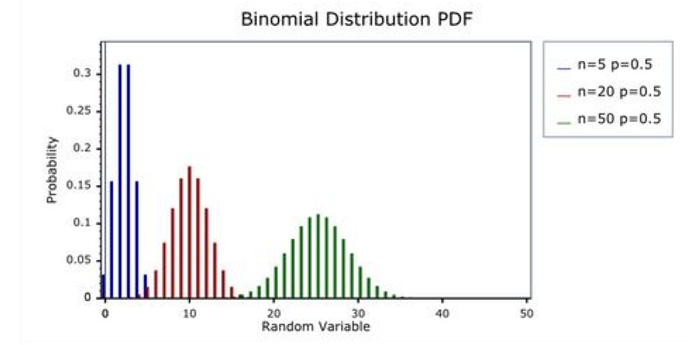
\includegraphics[width=1\linewidth]{images/binomial}

In another example, suppose that you will take 3 penalty kicks in a row.
The likelihood of making each penalty kick is ¾ or 75\%. What is the
probability that you will score 2 (and only 2) of the 3 penalty kicks?

\[fx(x)=  \binom{3}{x} .75^x (.25)^{3-x}\] P(X=0) = .02\\
P(X=1) = .14\\
P(X=2) = .42 \textless{}- this is the answer\\
P(X=3) = .42

\subsection{Properties of the Probability
Distribution}\label{properties-of-the-probability-distribution}

So for a general probability function, we have some broad properties:

\begin{itemize}
\tightlist
\item
  \(0 <= f_x(x_i) <= 1\) which is to say the value of any probability
  function is going to be between 0 and 1
\item
  \(Σ_i f_x (x_i) = 1\) if you sum up over all of the possible values it
  will sum to 1
\item
  \(P(A) = P(XcA) = Σ_Af_x(x_i)\) which is to say if you want the
  probability over a set of values of x, you just sum up the individual
  values for each item in the set
\end{itemize}

For a continous random variable, we rarely start with a verbal
description. Instead, we typically have a density that describes the
probability that the random variable is in various regions. The density,
or probability density function (PDF) is the continuous compliment to
the discrete PF. The PF (discret) and PDF (continous) are similar but
not exactly the same.

A random variable X is continuous if there exists a nonnegative function
f\_X\_ such that for any interval A c R as follows. We tend to speak
about a region, that A is in a region of the real line (R), the
probability that X is in A is equal to the integral over that region A
of the PDF.

\[P(X c A) = \int_{A} f_X(x)dx\]

\subsection{Discrete versus Continuous Random
Variables}\label{discrete-versus-continuous-random-variables}

Just like the discrete probability function, the probability density
function for a continous random variable has certain properties, these
are:

\begin{itemize}
\tightlist
\item
  \(0 <= f_X(x)\) which is to say it is non-negative. A PDF, unlike a
  PF, may have a region where the PDF is greater than 1\\
\item
  \(\int f_X(x) = 1\) the PF sums to one for each discreet part, the PDF
  integrates to one (as it is continous)
\item
  \(P(A) = P(a <= X <= b) = \int_{A} f_X(x)dx\) with discreet we sum for
  the values of interest, with PDF we integrate over the region (between
  a and b)
\end{itemize}

The value at a particular X for a PDF is equal to zero, if X is a
continous random variable.

In terms of point 1, we can think of it like the image below. The area
represented by the black lines will integrate to 1, however the area
under the red line will have a region (top left, above the line) where
it will integrate to more than 1.

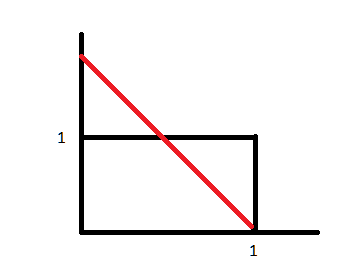
\includegraphics[width=1\linewidth]{images/PDF1}

In terms of any particular point (value of X) being zero, this is
because at any single point on a continuous random variable, it is
infinitely small and the integral of a single point is always zero. Or
from wikipedia (!):

\begin{quote}
Suppose a species of bacteria typically lives 4 to 6 hours. What is the
probability that a bacterium lives exactly 5 hours? The answer is 0\%. A
lot of bacteria live for approximately 5 hours, but there is no chance
that any given bacterium dies at exactly 5.0000000000\ldots{} hours.\\
Instead one might ask: What is the probability that the bacterium dies
between 5 hours and 5.01 hours? Suppose the answer is 0.02 (i.e., 2\%).
Next: What is the probability that the bacterium dies between 5 hours
and 5.001 hours? The answer should be about 0.002, since this time
interval is one-tenth as long as the previous. The probability that the
bacterium dies between 5 hours and 5.0001 hours should be about 0.0002,
and so on.\\
In these three examples, the ratio (probability of dying during an
interval) / (duration of the interval) is approximately constant, and
equal to 2 per hour (or 2 hour\^{}−1). For example, there is 0.02
probability of dying in the 0.01-hour interval between 5 and 5.01 hours,
and (0.02 probability / 0.01 hours) = 2 hour\^{}−1. This quantity 2
hour\^{}−1 is called the probability density for dying at around 5
hours.\\
Therefore, in response to the question ``What is the probability that
the bacterium dies at 5 hours?'', a literally correct but unhelpful
answer is ``0'', but a better answer can be written as (2 hour\^{}−1)dt.
This is the probability that the bacterium dies within a small
(infinitesimal) window of time around 5 hours, where dt is the duration
of this window.\\
For example, the probability that it lives longer than 5 hours, but
shorter than (5 hours + 1 nanosecond), is 2 hour\^{}−1⋅(1
nanosecond)≃6×10−13 (using the unit conversion 3.6×1012 nanoseconds = 1
hour).\\
There is a probability density function f with f(5hours)=2hour\^{}−1.
The integral of f over any window of time (not only infinitesimal
windows but also large windows) is the probability that the bacterium
dies in that window.
\end{quote}

\subsection{A Note on Terminology and the Uniform
Distribution}\label{a-note-on-terminology-and-the-uniform-distribution}

In both text books and online, there can be differences in both the the
terminology for random variables and the notation used. As noted
earlier, we tend to use PMF (or just PF) for discreet RVs, PDF for
continous and sometimes just PF or the ``distribution of a random
variable'' when talking more broadly about both. It's perhaps best just
to try and be consistent.

There can also be mixed random variables. One example might be if our
measuring technology is such that we cannot measure past a certain
point, so our variable is continous up to that point, then all values
beyond that point get truncated or grouped (it is a probability mass and
is discreet) to that maximal value.

There are some random variables which are simply uniform. We call such a
random variable X ``uniform with parameters and b'' denoted as
\(X \sim U[a,b]\). In such a situation, the probability of X is defined
in such a way that the probability of X belonging to any subinterval of
X is proportional to the length of the subinterval. Graphically, it
looks like a box and similar to the last image above (the black line).

To calculate the probability of some interval {[}c,d{]} in {[}a,b{]} you
integrate a/(b-a) over that region, or as the PDF is flat, we can just
use (d-c)/(b-a). e.g.~if we have a random variable that is
uniformly-distributed from 3 to 8. What is the probability that the
random variable takes on a value less than or equal to 7?

(7-3) / (8-3) = 4/5 = 0.8 or 80\%

\subsection{The Cumulative Distribution
Function}\label{the-cumulative-distribution-function}

Both discreet and continous random variables can be expressed in the
form of a continous random variable (CDF) which takes on a value between
0 and 1. It is defined as:

\[f_X(x) = P(X <= x)\] Also note that \(lim_{x→-∞}\; FX(x) = 0\)\\
\(lim_{x→∞}\; FX(x) = 1\)

So the CDF will start at zero, it may have flat parts, but it will never
decrease. And as we go to the limit (x approaches infinity) then the CDF
will be equal to 1.

Given a CDF it would be possible to recover the PDF or PF for continous
or discreet distribution respectively.

\begin{itemize}
\tightlist
\item
  So if you want to get the CDF for a continuous random variable at a
  particular point, then you integrate the PDF up to that point:
  \(FX (x) = P(X <= x) = -∞∫ fX(x)dx\)
\item
  If you have the CDF and you want to get the PDF i.e.~you want to
  recover the PDF from it, then you take the derivative:
  \(F’X(x) = \frac{dF(x)}{dx} = fX(x)\)
\end{itemize}

\subsection{Joint Distributions}\label{joint-distributions}

A lot of what we do in data analysis is gather repeated observations
from joint distributions of random variables, for instance, rainfall and
crop growth. Such a two way joint distribution is called a bivariate
distribution.

More formally we say

If X and Y are continuous random variables defined on the same sample
space S, then the joint probability density function of X\&Y,
f\_X\_Y(x,y), is the surface such that for any region A of the xy-plane
- note this is similar to the generalisation of the PDF but as a
generalisation of the bivariate distribution:

\[P((X,Y) c A) = ∫∫AfXY(x,y)dxdy\] Like the PDF from before, it will
integrate over the entire area to 1, and the probability at any one
particular point is equal to zero.

*\href{https://www.youtube.com/watch?v=w97tr8dafGA}{Video on single and
double integration including limit}

\subsection{Joint Distribution
Example}\label{joint-distribution-example}

If you develop a headache you might decide to take tablets, one may be
paracetamol and the other ibuprofen. If X is the effective period of
ipbuprofen and Y that of paracetamol, then

\[fXY(x,y) = λ^2exp{-λ(x+y)} \; \; for x,y >= 0\]

Lambda is introducting some function - it is a general formula or `black
box', it states how the output calculated in relation to the input.

\href{https://www.youtube.com/watch?v=eis11j_iGMs}{Lambda Calculus}
\href{https://en.wikipedia.org/wiki/Church\%E2\%80\%93Turing_thesis}{Church-Turing
Hypothesis}
\href{https://en.wikipedia.org/wiki/List_of_integrals_of_exponential_functions\#Integrals_involving_only_exponential_functions}{Integrals
for exponential functions}

In this case, lambda can be considered as a constant, so our steps would
be

\begin{itemize}
\tightlist
\item
  remove λ i.e.~let λ=1 and work just on \(exp{-λ(x+y)}\)\\
\item
  integrate on Y from {[}0,3{]} (meaning x is just another constant)\\
\item
  without Y, integrate on X from {[}0,3{]}
\end{itemize}

We could always put λ back in later.

In our example, we are interested in the probability that the medicine
is effective within 3 hours, however we wish to calculate the
probability that the headache comes back within three hours (or less),
so we have a double integration to calculate the area over which it is
effective (3 hours), then the probability becomes 1 minus that area (the
probability it comes back). e.g.

\$ \int\emph{\{0\}\^{}\{3\} \int}\{0\}\^{}\{3\}
λ\^{}2exp\{-λ(x+y)\}dydx\$\\
\ldots{}calculation steps\\
\((1-exp({-3λ})^2\)

The area we calculate is roughly shown as below - not there should be an
area above the axis also, not just a 2d plane

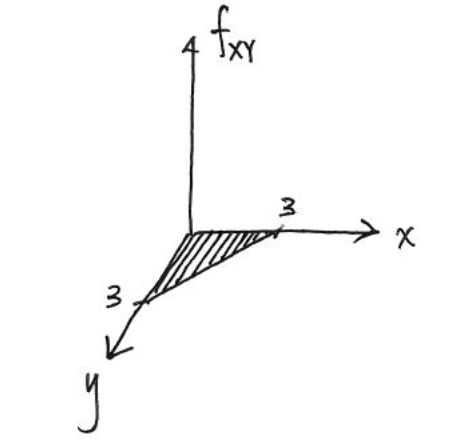
\includegraphics[width=1\linewidth]{images/headache}

The calculation steps missed out are as follows:

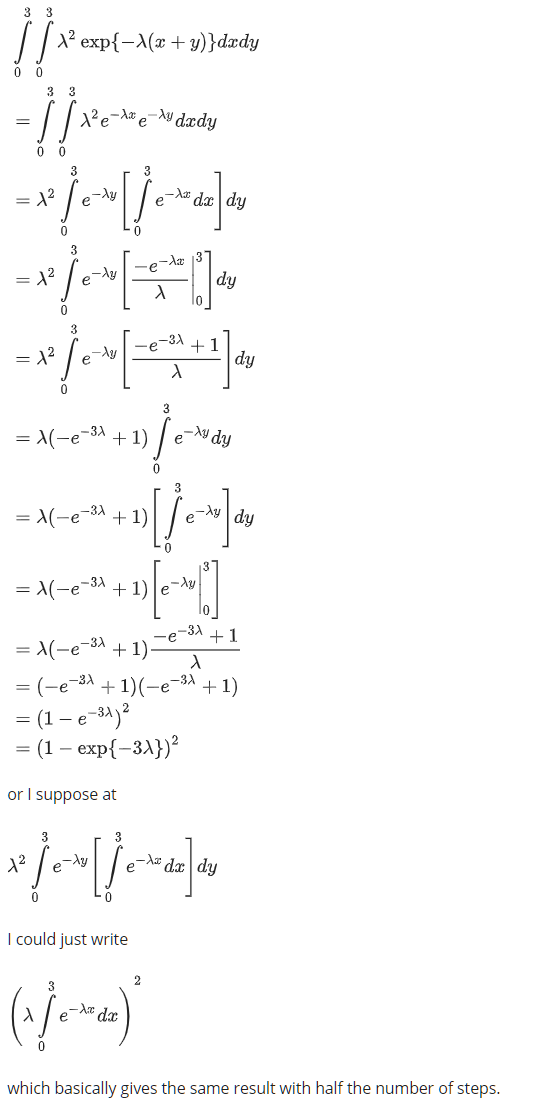
\includegraphics[width=1\linewidth]{images/headachesteps}

If we change the question so that we take the paracetamol only after the
ibuprofen has stopped working, what is the probability the sum of the
two lengths is less than or equal to three. The region over which we
integrate over changes

\$ \int\_\{0\}\^{}\{3\}{[} \int\_\{0\}\^{}\{3-x\} λ\^{}2 ;
exp\^{}\{-λx\} ; exp\^{}\{-λy\} dy{]}dx\$\\
\ldots{}\\
\(1-(1 + 3λ) e^{-3λ}\)

The joint probability is the result of two random variables which are
independent, which means you multiply their individual distributions
together.

If we wanted to take one drug then the other - sequentially - we could
work out the total effective length as Z. What is FZ(z) = P(Z
\textless{}= z) = P(X+Y \textless{}= z). We take the derivative fZ(z) =
F'Z(z) = \(λ^2zexp(- zλ)\), for z \textgreater{} 0.

\begin{itemize}
\tightlist
\item
  The study of statistics is essentially functions of random variables.
  And so if we want to understand how statistics behave, we have to
  understand how functions of random variables behave.
\end{itemize}

\section{Gathering and Collecting
Data}\label{gathering-and-collecting-data}

We essentially have three data sources:

\begin{enumerate}
\def\labelenumi{\arabic{enumi}.}
\tightlist
\item
  Existing data libraries - collected by someone else\\
\item
  Collect your own\\
\item
  Extracting data from the internet - really this means generating data,
  since 1 could be from the internet
\end{enumerate}

There are a lot of data sources available on the web for social
sciences, including international census
\href{https://international.ipums.org/international/}{IPUMS} and others:

A Great resource for MIT students and others:
\url{http://libguides.mit.edu/ssds}\\
Amazon dataverse \url{http://aws.amazon.com/public-data-sets/}\\
\href{http://www.icpsr.umich.edu/icpsrweb/ICPSR/}{ICPSR which includes
published guidelines for handling identifiable information and for
documenting datasets publishing data such as codebooks etc}\\
Plus more - \href{./files/M1/Gathering_Data.pdf}{see slide 3}

We can also use DHS harmonised questions and datasets on
\href{http://www.dhsprogram.com/}{demographic and health}.

Additionally, more and more social scientists and national governments
are running expriments or RTCs and then making the trial data available
online after. Harvard publish their RCT findings and sometimes data in
thier
\href{https://dataverse.harvard.edu/dataverse/socialsciencercts}{RCT
dataverse}. The use of data collected for a specific purpose, including
RCTs, is used less by secondary researchers than other datasets e.g.~LFS
style surveys. Many journals now require publishing of datasets, such as
the The American Economic Association journals, however these datasets
are published more for transparency purposes rather than data re-use.

There are more links to data sources on the slides.

\subsection{A Google Maps API example}\label{a-google-maps-api-example}

The Google API allows search of up to 2,500 per day for free, then about
£1 per 2000 after that, as a researcher therefore it is possible to do
queries over multiple days to get your dataset and not be charged.

USing Google Maps it is possible to get travel times from point A to
point B, taking into account traffic conditions. This data is obtained
via crowdsourced Google Android users. It is possible to get both
departure time now results - API call is ?now - or depature time
predictions based on historic trends - API call ?prediction.

An example of the departure time now API call was the Delhi Odd-Even
study - there was a restriction on driving with certain number plates on
certain days. Delhi is one of the most polluted cities in the world.
They initially implemented the policy for a 15 day period of January 1st
to 15th 2016. So a researcher collected data from the 1st January 2016
for 93 routes across Delhi, every 20 minutes, for the 15 days of the
policy then 15 days after the policy.

\subsection{Web Scraping}\label{web-scraping}

Data is not always available via an API, but we still have the web page.
Ellison and Ellison (as in the teacher of this class with her husband)
did some research to look at the prices of used books online compared to
bricks and mortar stores. Abebooks was used as a the online data source.
We can extract = web scrape - the price data by extracting the relevant
code blocks from the returned results. We would use BeautifulSoup
library in Python to pull up the search on the identified page then
bring up the class - span class - element which contains the price.
BeautifulSoup is a simple Python package which allows users to find
information on websites by utilizing a site's HTML or XML code.

We can also do webscraping in R. R is fine as long as the webscraping
project is not very large. We use the package rvest which works well
with the Chrome Plugin called Selector Gadget. An example might be to
get admissions data from CalPoly via a html page on their site e.g.

\begin{Shaded}
\begin{Highlighting}[]
\CommentTok{# Note there was an error in the original slides and handout, whereby the code printed each object to the console, then saved all tables in to a html file}
\CommentTok{# I believe the intention was to save each html table in to it's own object so you have three extracted html tables, rather than three}
\CommentTok{# identical objects each containing all three tables}

\KeywordTok{library}\NormalTok{(rvest)}
\end{Highlighting}
\end{Shaded}

\begin{verbatim}
## Loading required package: xml2
\end{verbatim}

\begin{Shaded}
\begin{Highlighting}[]
\NormalTok{CPadmissions <-}\StringTok{ }\KeywordTok{read_html}\NormalTok{(}\StringTok{"https://admissions.calpoly.edu/prospective/profile.html"}\NormalTok{)}

\NormalTok{admission_}\DecValTok{1}\NormalTok{ <-}\StringTok{ }\NormalTok{CPadmissions }\OperatorTok
\StringTok{  }\KeywordTok{html_nodes}\NormalTok{(}\StringTok{"table"}\NormalTok{) }\OperatorTok
\StringTok{  }\NormalTok{.[[}\DecValTok{1}\NormalTok{]] }\OperatorTok
\StringTok{  }\KeywordTok{html_table}\NormalTok{()}

\NormalTok{admission_}\DecValTok{2}\NormalTok{ <-}\StringTok{ }\NormalTok{CPadmissions }\OperatorTok
\StringTok{  }\KeywordTok{html_nodes}\NormalTok{(}\StringTok{"table"}\NormalTok{) }\OperatorTok
\StringTok{  }\NormalTok{.[[}\DecValTok{2}\NormalTok{]] }\OperatorTok
\StringTok{  }\KeywordTok{html_table}\NormalTok{()}

\NormalTok{admission_}\DecValTok{3}\NormalTok{ <-}\StringTok{ }\NormalTok{CPadmissions }\OperatorTok
\StringTok{  }\KeywordTok{html_nodes}\NormalTok{(}\StringTok{"table"}\NormalTok{) }\OperatorTok
\StringTok{  }\NormalTok{.[[}\DecValTok{3}\NormalTok{]] }\OperatorTok
\StringTok{  }\KeywordTok{html_table}\NormalTok{()}

\NormalTok{admission_}\DecValTok{1}
\end{Highlighting}
\end{Shaded}

\begin{verbatim}
##                                      COLLEGE APPLIED SELECTED Target  GPA
## 1 Agriculture, Food & Environmental Sciences   4,842    2,150    907 4.00
## 2        Architecture & Environmental Design   2,453      929    404 4.02
## 3                                   Business   7,105    2,271    655 4.12
## 4                                Engineering  19,071    4,337  1,123 4.21
## 5                               Liberal Arts   9,265    3,025    756 4.04
## 6                      Science & Mathematics  11,923    3,753    641 4.18
## 7                                      TOTAL  54,659   16,465  4,486 4.12
##   ACT* SAT*
## 1   28 1325
## 2   29 1364
## 3   30 1410
## 4   32 1481
## 5   29 1355
## 6   31 1420
## 7   30 1407
\end{verbatim}

\begin{Shaded}
\begin{Highlighting}[]
\NormalTok{admission_}\DecValTok{2}
\end{Highlighting}
\end{Shaded}

\begin{verbatim}
##                                      COLLEGE APPLIED SELECTED Target  GPA
## 1 Agriculture, Food & Environmental Sciences   1,008      283    172 3.28
## 2        Architecture & Environmental Design     408       86     56 3.24
## 3                                   Business   2,323      247    118 3.56
## 4                                Engineering   2,978      395    203 3.47
## 5                               Liberal Arts   2,771      443    185 3.41
## 6                      Science & Mathematics   1,434      260    117 3.41
## 7                                      TOTAL  10,922    1,714    893 3.41
\end{verbatim}

\begin{Shaded}
\begin{Highlighting}[]
\NormalTok{admission_}\DecValTok{3}
\end{Highlighting}
\end{Shaded}

\begin{verbatim}
##                                      COLLEGE UNDERGRAD POSTBAC/GRAD  TOTAL
## 1 Agriculture, Food & Environmental Sciences     4,079           78  4,157
## 2        Architecture & Environmental Design     1,827           46  1,873
## 3                                   Business     3,051           45  3,096
## 4                                Engineering     5,996          292  6,288
## 5                               Liberal Arts     3,309           92  3,401
## 6                      Science & Mathematics     2,786          317  3,103
## 7                                     Others        44           17     61
## 8                                      TOTAL    21,092          887 21,979
\end{verbatim}

Comment from another student was `if you want to get good at web
scraping learn xpath and also css selectors. If you plan on working with
xml data xpath is a must'.

Another example where we want specific items would be as follows, we
find out which elements we need from the webpage (search results in this
instance) using the selector gadget.

\begin{Shaded}
\begin{Highlighting}[]
\KeywordTok{library}\NormalTok{(rvest)}

\NormalTok{link <-}\StringTok{ "https://www.abebooks.co.uk/servlet/SearchResults?sts=t&cm_sp=SearchF-_-home-_-Results&an=&tn=&kn=&isbn=2070361594"}
\NormalTok{larecherche <-}\StringTok{ }\KeywordTok{read_html}\NormalTok{(link)}

\NormalTok{titlehtml <-}\StringTok{ }\KeywordTok{html_nodes}\NormalTok{(larecherche, }\StringTok{".col-xs-8 a span"}\NormalTok{)}
\NormalTok{titletext <-}\StringTok{ }\KeywordTok{html_text}\NormalTok{(titlehtml)}

\NormalTok{pricehtml <-}\StringTok{ }\KeywordTok{html_nodes}\NormalTok{(larecherche, }\StringTok{".item-price .price"}\NormalTok{)}
\NormalTok{pricetext <-}\StringTok{ }\KeywordTok{html_text}\NormalTok{(pricehtml)}

\KeywordTok{head}\NormalTok{(pricetext)}
\end{Highlighting}
\end{Shaded}

\begin{verbatim}
## [1] "£ 2.59" "£ 3.30" "£ 0.76" "£ 0.84" "£ 2.99" "£ 5.50"
\end{verbatim}

Note that the results are in ascending order - lowest priced overall -
first. The reason that some later ones are lower price is that it does
not include shipping in the results, that is a seperate item in the
html. We should therefore consider extracting the shipping item also,
then combining the two data tables together to give a total price.

We can also write slightly cleaner code using the pipe operator as
follows.

\begin{Shaded}
\begin{Highlighting}[]
\KeywordTok{library}\NormalTok{(rvest)}
\KeywordTok{library}\NormalTok{(tidyr)}
\KeywordTok{library}\NormalTok{(dplyr)}
\end{Highlighting}
\end{Shaded}

\begin{verbatim}
## 
## Attaching package: 'dplyr'
\end{verbatim}

\begin{verbatim}
## The following objects are masked from 'package:stats':
## 
##     filter, lag
\end{verbatim}

\begin{verbatim}
## The following objects are masked from 'package:base':
## 
##     intersect, setdiff, setequal, union
\end{verbatim}

\begin{Shaded}
\begin{Highlighting}[]
\NormalTok{larecherche <-}\StringTok{ }\KeywordTok{read_html}\NormalTok{(link)}

\NormalTok{price <-}\StringTok{ }\NormalTok{larecherche }\OperatorTok
\StringTok{  }\KeywordTok{html_nodes}\NormalTok{(}\StringTok{".item-price .price"}\NormalTok{) }\OperatorTok
\StringTok{  }\KeywordTok{html_text}\NormalTok{() }\OperatorTok
\StringTok{  }\NormalTok{readr}\OperatorTok{::}\KeywordTok{parse_number}\NormalTok{()}

\NormalTok{booktitle <-}\StringTok{ }\NormalTok{larecherche }\OperatorTok
\StringTok{  }\KeywordTok{html_nodes}\NormalTok{(}\StringTok{".col-xs-8 a span"}\NormalTok{) }\OperatorTok
\StringTok{  }\KeywordTok{html_text}\NormalTok{() }\OperatorTok
\StringTok{  }\NormalTok{readr}\OperatorTok{::}\KeywordTok{parse_character}\NormalTok{()}

\NormalTok{combined <-}\StringTok{ }\KeywordTok{data_frame}\NormalTok{(booktitle, }\StringTok{'data and time'}\NormalTok{ =}\StringTok{ }\KeywordTok{Sys.time}\NormalTok{(), price)}

\KeywordTok{head}\NormalTok{(combined)}
\end{Highlighting}
\end{Shaded}

\begin{verbatim}
## # A tibble: 6 x 3
##   booktitle                                      `data and time`     price
##   <chr>                                          <dttm>              <dbl>
## 1 Le temps retrouve                              2018-10-17 19:50:27  2.59
## 2 Le temps retrouve                              2018-10-17 19:50:27  3.3 
## 3 Le temps retrouve                              2018-10-17 19:50:27  0.76
## 4 Le temps retrouve                              2018-10-17 19:50:27  0.84
## 5 À la recherche du temps perdu : Le temps retr~ 2018-10-17 19:50:27  2.99
## 6 À la recherche du temps perdu : Le temps retr~ 2018-10-17 19:50:27  5.5
\end{verbatim}

If you collect your own data, sometimes in an academic environment you
may need to complete a process to authenticate the data collection
method. This would be an Institutional Review Board or IRB at MIT who
would check your data collection method is ethical. Sometimes these are
called more generically Human Research Board or just an ethics
committee. They may be national guidance governing ethical
considerations and research involving humans. In the UK there are the
ESRC Framework for Research Ethics for instance.

\subsection{Human Research Subject
Definitions}\label{human-research-subject-definitions}

\emph{Research} - A systematic investigation, including research
development, testing and evaluation, designed to develop or contribute
to generalizable knowledge. \textbf{This means that Facebook or Amazon
can experiment as much as they want on you unless they publish; but if
you are working with them with the goal of publishing you need to go
through an IRB}

\emph{Human Subject} - A living individual about whom an investigator
(whether professional or student) conducting research obtains (1) data
through intervention or interaction with the individual, or (2)
identifiable private information.

\section{Homework}\label{homework}

This is a sample of some of the homework answers.

Q9

\begin{Shaded}
\begin{Highlighting}[]
\NormalTok{success <-}\StringTok{ }\KeywordTok{rbinom}\NormalTok{(}\DecValTok{1000}\NormalTok{, }\DecValTok{8}\NormalTok{, }\FloatTok{0.2}\NormalTok{)}
\KeywordTok{hist}\NormalTok{(success)}
\end{Highlighting}
\end{Shaded}

\includegraphics{Module2_files/figure-latex/unnamed-chunk-5-1.pdf}

Q12 A. What is the probability of getting exactly 7 heads on 10 flips?

dbinom() function gives the probability density distribution at each
point.

\begin{Shaded}
\begin{Highlighting}[]
\CommentTok{# Calculate the figure}
\KeywordTok{dbinom}\NormalTok{(}\DecValTok{7}\NormalTok{,}\DecValTok{10}\NormalTok{,}\FloatTok{0.65}\NormalTok{)}
\end{Highlighting}
\end{Shaded}

\begin{verbatim}
## [1] 0.2522196
\end{verbatim}

\begin{Shaded}
\begin{Highlighting}[]
\CommentTok{#Plot the distribution}
\NormalTok{x <-}\StringTok{ }\KeywordTok{seq}\NormalTok{(}\DecValTok{1}\NormalTok{,}\DecValTok{10}\NormalTok{,}\DataTypeTok{by =} \DecValTok{1}\NormalTok{)}
\NormalTok{y <-}\StringTok{ }\KeywordTok{dbinom}\NormalTok{(x,}\DecValTok{10}\NormalTok{,}\FloatTok{0.65}\NormalTok{)}
\KeywordTok{plot}\NormalTok{(x,y)}
\end{Highlighting}
\end{Shaded}

\includegraphics{Module2_files/figure-latex/unnamed-chunk-6-1.pdf}

B. What is the probability of getting at most 7 heads on 10 flips?

\begin{Shaded}
\begin{Highlighting}[]
\CommentTok{# Probability of getting 7 or less heads from 10 tosses of a coin}
\KeywordTok{pbinom}\NormalTok{(}\DecValTok{7}\NormalTok{,}\DecValTok{10}\NormalTok{,}\FloatTok{0.65}\NormalTok{)}
\end{Highlighting}
\end{Shaded}

\begin{verbatim}
## [1] 0.7383926
\end{verbatim}

C.What is the probability of getting at least 6 heads on 10 flips?

\begin{Shaded}
\begin{Highlighting}[]
\CommentTok{# Probability of getting 6 or greater heads from 10 tosses of a coin}
\KeywordTok{pbinom}\NormalTok{(}\DecValTok{5}\NormalTok{,}\DecValTok{10}\NormalTok{,}\FloatTok{0.65}\NormalTok{, }\DataTypeTok{lower.tail =}\NormalTok{ F)}
\end{Highlighting}
\end{Shaded}

\begin{verbatim}
## [1] 0.7514955
\end{verbatim}

Q14. - Tidy up the R code and fill in the blanks

\begin{Shaded}
\begin{Highlighting}[]
\KeywordTok{library}\NormalTok{(dplyr)}
\KeywordTok{library}\NormalTok{(tibble)}
\KeywordTok{library}\NormalTok{(ggplot2)}

\NormalTok{binom_draws <-}\StringTok{ }\KeywordTok{as_tibble}\NormalTok{(}\KeywordTok{data.frame}\NormalTok{(success))}

\NormalTok{estimated_pf <-}\StringTok{ }\NormalTok{binom_draws }\OperatorTok
\StringTok{  }\KeywordTok{group_by}\NormalTok{(success) }\OperatorTok
\StringTok{  }\KeywordTok{summarise}\NormalTok{(}\DataTypeTok{n=}\KeywordTok{n}\NormalTok{()) }\OperatorTok
\StringTok{  }\KeywordTok{mutate}\NormalTok{(}\DataTypeTok{freq =}\NormalTok{ n}\OperatorTok{/}\KeywordTok{sum}\NormalTok{(n))}

\KeywordTok{ggplot}\NormalTok{(estimated_pf, }\KeywordTok{aes}\NormalTok{(success, freq)) }\OperatorTok{+}\StringTok{ }
\StringTok{  }\KeywordTok{geom_col}\NormalTok{() }\OperatorTok{+}
\StringTok{  }\KeywordTok{ylab}\NormalTok{(}\StringTok{"Estimated Density"}\NormalTok{)}
\end{Highlighting}
\end{Shaded}

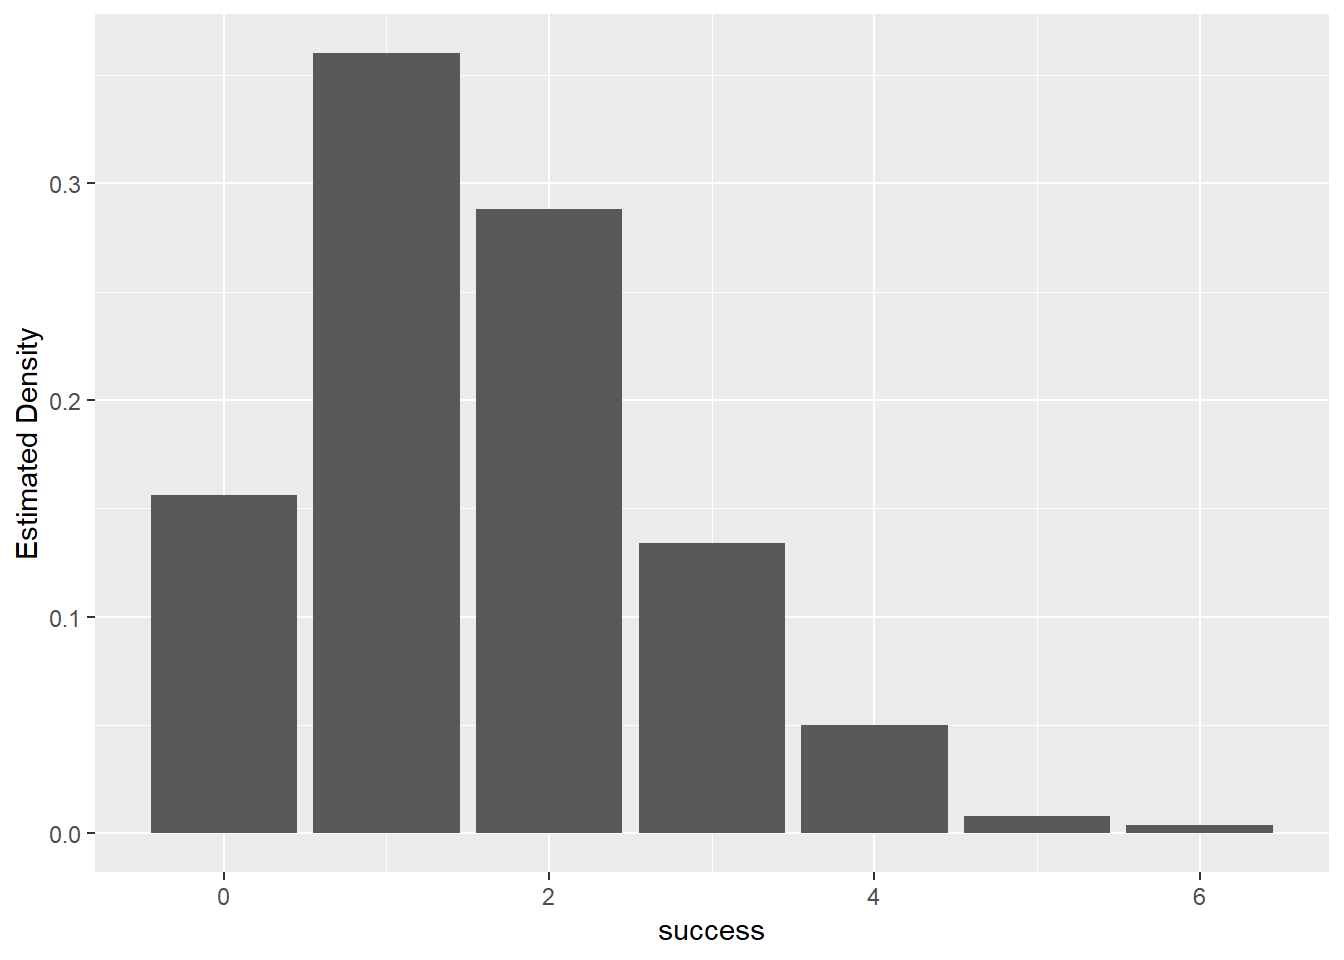
\includegraphics{Module2_files/figure-latex/unnamed-chunk-9-1.pdf}

\chapter{Module 3: Describing Data, Joint and Conditional Distributions
of Random
Variables}\label{module-3-describing-data-joint-and-conditional-distributions-of-random-variables}

\begin{center}\rule{0.5\linewidth}{\linethickness}\end{center}

\textbf{Module Sections:}

\begin{itemize}
\tightlist
\item
  Summarizing and Describing Data
\item
  Joint, Marginal, and Conditional Distributions
\item
  R Tutorials: Basic Functions
\item
  Module 3: Homework
\end{itemize}

Module Content:

\begin{itemize}
\tightlist
\item
  \href{./files/M3/SummarizingandDescribingDataSlides.pdf}{Summarizing
  and Describing Data Slides}
\end{itemize}

\section{Summarizing and Describing
Data}\label{summarizing-and-describing-data}

The goal of visualisation is either EDA for yourself or for conveying a
message to other people. The course uses ggplot in both instances, this
module focuses more on EDA for yourself.

One common way of initially looking at the data is to use a histogram,
which provides a rough estimate of the probability distribution function
(PDF) of a continous variable. We can have right open or closed sets
when creating histogram bins \([a_i,b_i), [a_{i+1},b_{i+1})\) see this
video for a \href{https://youtu.be/kREoWbByNZs}{discussion on binning}.

\begin{Shaded}
\begin{Highlighting}[]
\KeywordTok{library}\NormalTok{(ggplot2)}
\KeywordTok{require}\NormalTok{(cowplot)}
\end{Highlighting}
\end{Shaded}

\begin{verbatim}
## Loading required package: cowplot
\end{verbatim}

\begin{verbatim}
## 
## Attaching package: 'cowplot'
\end{verbatim}

\begin{verbatim}
## The following object is masked from 'package:ggplot2':
## 
##     ggsave
\end{verbatim}

\begin{Shaded}
\begin{Highlighting}[]
\KeywordTok{library}\NormalTok{(tidyverse)}
\end{Highlighting}
\end{Shaded}

\begin{verbatim}
## -- Attaching packages ------------------ tidyverse 1.2.1 --
\end{verbatim}

\begin{verbatim}
## v tibble  1.4.2     v purrr   0.2.5
## v tidyr   0.8.1     v dplyr   0.7.6
## v readr   1.1.1     v stringr 1.3.1
## v tibble  1.4.2     v forcats 0.3.0
\end{verbatim}

\begin{verbatim}
## -- Conflicts --------------------- tidyverse_conflicts() --
## x dplyr::filter()   masks stats::filter()
## x cowplot::ggsave() masks ggplot2::ggsave()
## x dplyr::lag()      masks stats::lag()
\end{verbatim}

\begin{Shaded}
\begin{Highlighting}[]
\NormalTok{bihar_data <-}\StringTok{ }\KeywordTok{read_csv}\NormalTok{(}\StringTok{"./files/M3/Bihar.csv"}\NormalTok{)}
\end{Highlighting}
\end{Shaded}

\begin{verbatim}
## Parsed with column specification:
## cols(
##   personid = col_integer(),
##   female = col_integer(),
##   adult = col_integer(),
##   age = col_double(),
##   height_cm = col_double(),
##   weight_kg = col_double()
## )
\end{verbatim}

\begin{Shaded}
\begin{Highlighting}[]
\CommentTok{# keep the females}
\NormalTok{bihar_adult_females <-}\StringTok{ }\NormalTok{dplyr}\OperatorTok{::}\KeywordTok{filter}\NormalTok{(bihar_data, adult }\OperatorTok{==}\StringTok{ }\DecValTok{1}\NormalTok{, female }\OperatorTok{==}\StringTok{ }\DecValTok{1}\NormalTok{)}

\CommentTok{# take a look at our data}
\KeywordTok{head}\NormalTok{(bihar_adult_females, }\DecValTok{10}\NormalTok{)}
\end{Highlighting}
\end{Shaded}

\begin{verbatim}
## # A tibble: 10 x 6
##    personid female adult   age height_cm weight_kg
##       <int>  <int> <int> <dbl>     <dbl>     <dbl>
##  1 11010103      1     1    28      150.      37.7
##  2 11010202      1     1    30      140.      57.3
##  3 11010207      1     1    35      148.      38.9
##  4 11010302      1     1    48      145.      35.7
##  5 11010303      1     1    22       NA       NA  
##  6 11010306      1     1    18       NA       NA  
##  7 11010308      1     1    28      145.      42.4
##  8 11010402      1     1    58      156.      51.1
##  9 11010404      1     1    36      156.      50.7
## 10 11010407      1     1    55      156.      47.2
\end{verbatim}

\begin{Shaded}
\begin{Highlighting}[]
\CommentTok{# plot it}
\KeywordTok{ggplot}\NormalTok{(bihar_adult_females, }\KeywordTok{aes}\NormalTok{(height_cm)) }\OperatorTok{+}\StringTok{ }
\StringTok{  }\KeywordTok{geom_histogram}\NormalTok{()}
\end{Highlighting}
\end{Shaded}

\begin{verbatim}
## `stat_bin()` using `bins = 30`. Pick better value with `binwidth`.
\end{verbatim}

\begin{verbatim}
## Warning: Removed 1432 rows containing non-finite values (stat_bin).
\end{verbatim}

\includegraphics{Module3_files/figure-latex/unnamed-chunk-1-1.pdf}

\begin{Shaded}
\begin{Highlighting}[]
\CommentTok{# not very attractive, so lets tidy it up - there are some outliers close to 0 and 200 cm}
\NormalTok{bihar_adult_females_trunc <-}\StringTok{ }\NormalTok{dplyr}\OperatorTok{::}\KeywordTok{filter}\NormalTok{(bihar_adult_females, height_cm }\OperatorTok{>}\StringTok{ }\DecValTok{120}\NormalTok{, height_cm }\OperatorTok{<}\StringTok{ }\DecValTok{200}\NormalTok{)}

\CommentTok{# Plot again with colour and labels}
\KeywordTok{ggplot}\NormalTok{(bihar_adult_females_trunc, }\KeywordTok{aes}\NormalTok{(height_cm)) }\OperatorTok{+}\StringTok{ }
\StringTok{  }\KeywordTok{geom_histogram}\NormalTok{(}\DataTypeTok{fill =} \StringTok{"blue"}\NormalTok{, }\DataTypeTok{color =} \StringTok{"darkblue"}\NormalTok{) }\OperatorTok{+}\StringTok{ }
\StringTok{  }\KeywordTok{xlab}\NormalTok{(}\StringTok{"Height in centimeters, Bihar Females (truncated)"}\NormalTok{)}
\end{Highlighting}
\end{Shaded}

\begin{verbatim}
## `stat_bin()` using `bins = 30`. Pick better value with `binwidth`.
\end{verbatim}

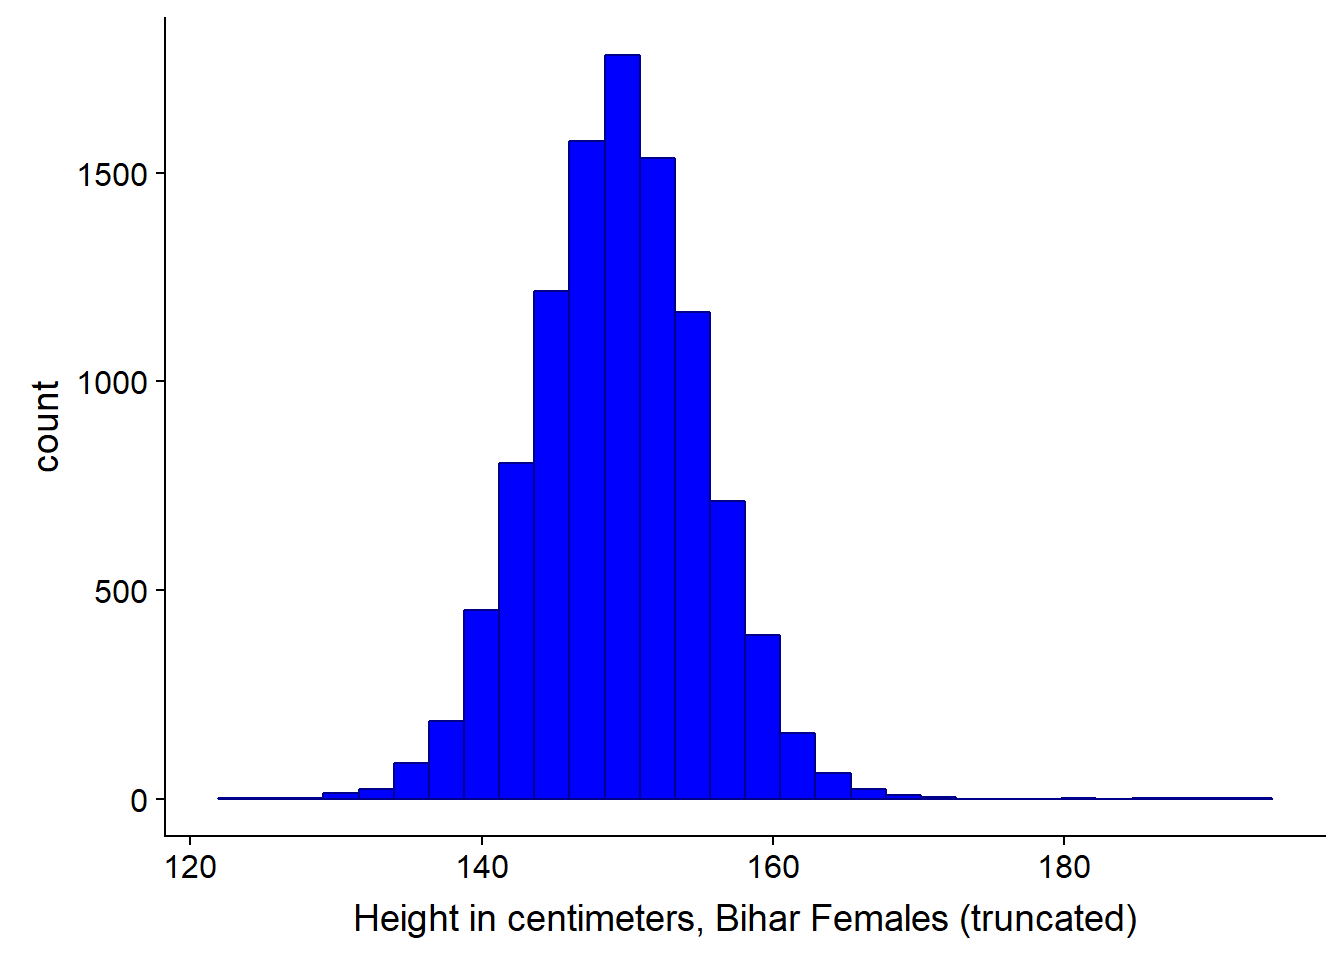
\includegraphics{Module3_files/figure-latex/unnamed-chunk-1-2.pdf}

We could also adjust the bin width at this point if we wanted to. The
width of the bins depends in part on the volume of data you have, for
instance, if you have just 50 observations, picking bin widths of 1 cm
might be too much - you can't be sure your data is reliable, there may
be quite a lot of noise. Conversely, if you have a million observations,
1 cm bin widths might be fine.

\begin{Shaded}
\begin{Highlighting}[]
\NormalTok{Bihar1 <-}\StringTok{ }\KeywordTok{ggplot}\NormalTok{(bihar_adult_females_trunc, }\KeywordTok{aes}\NormalTok{(height_cm)) }\OperatorTok{+}\StringTok{ }
\StringTok{  }\KeywordTok{geom_histogram}\NormalTok{(}\DataTypeTok{fill =} \StringTok{"blue"}\NormalTok{,}\DataTypeTok{color =} \StringTok{"darkblue"}\NormalTok{, }\DataTypeTok{binwidth =} \DecValTok{5}\NormalTok{) }\OperatorTok{+}
\StringTok{  }\KeywordTok{xlab}\NormalTok{(}\StringTok{"binwidth = 5"}\NormalTok{)}

\NormalTok{Bihar2 <-}\StringTok{ }\KeywordTok{ggplot}\NormalTok{(bihar_adult_females_trunc, }\KeywordTok{aes}\NormalTok{(height_cm)) }\OperatorTok{+}\StringTok{ }
\StringTok{  }\KeywordTok{geom_histogram}\NormalTok{(}\DataTypeTok{fill =} \StringTok{"blue"}\NormalTok{,}\DataTypeTok{color =} \StringTok{"darkblue"}\NormalTok{, }\DataTypeTok{binwidth =} \DecValTok{10}\NormalTok{) }\OperatorTok{+}
\StringTok{  }\KeywordTok{xlab}\NormalTok{(}\StringTok{"binwidth = 10"}\NormalTok{)}

\NormalTok{Bihar3 <-}\StringTok{ }\KeywordTok{ggplot}\NormalTok{(bihar_adult_females_trunc, }\KeywordTok{aes}\NormalTok{(height_cm)) }\OperatorTok{+}\StringTok{ }
\StringTok{  }\KeywordTok{geom_histogram}\NormalTok{(}\DataTypeTok{fill =} \StringTok{"blue"}\NormalTok{,}\DataTypeTok{color =} \StringTok{"darkblue"}\NormalTok{, }\DataTypeTok{binwidth =} \DecValTok{20}\NormalTok{) }\OperatorTok{+}
\StringTok{  }\KeywordTok{xlab}\NormalTok{(}\StringTok{"binwidth = 20"}\NormalTok{)}

\NormalTok{Bihar4 <-}\StringTok{ }\KeywordTok{ggplot}\NormalTok{(bihar_adult_females_trunc, }\KeywordTok{aes}\NormalTok{(height_cm)) }\OperatorTok{+}\StringTok{ }
\StringTok{  }\KeywordTok{geom_histogram}\NormalTok{(}\DataTypeTok{fill =} \StringTok{"blue"}\NormalTok{,}\DataTypeTok{color =} \StringTok{"darkblue"}\NormalTok{, }\DataTypeTok{binwidth =} \DecValTok{50}\NormalTok{) }\OperatorTok{+}
\StringTok{  }\KeywordTok{xlab}\NormalTok{(}\StringTok{"binwidth = 50"}\NormalTok{)}

\KeywordTok{plot_grid}\NormalTok{(Bihar1, Bihar2, Bihar3, Bihar4, }\DataTypeTok{labels=}\StringTok{"female height in Bihar"}\NormalTok{, }\DataTypeTok{hjust =} \OperatorTok{-}\DecValTok{1}\NormalTok{, }\DataTypeTok{vjust =} \DecValTok{1}\NormalTok{)}
\end{Highlighting}
\end{Shaded}

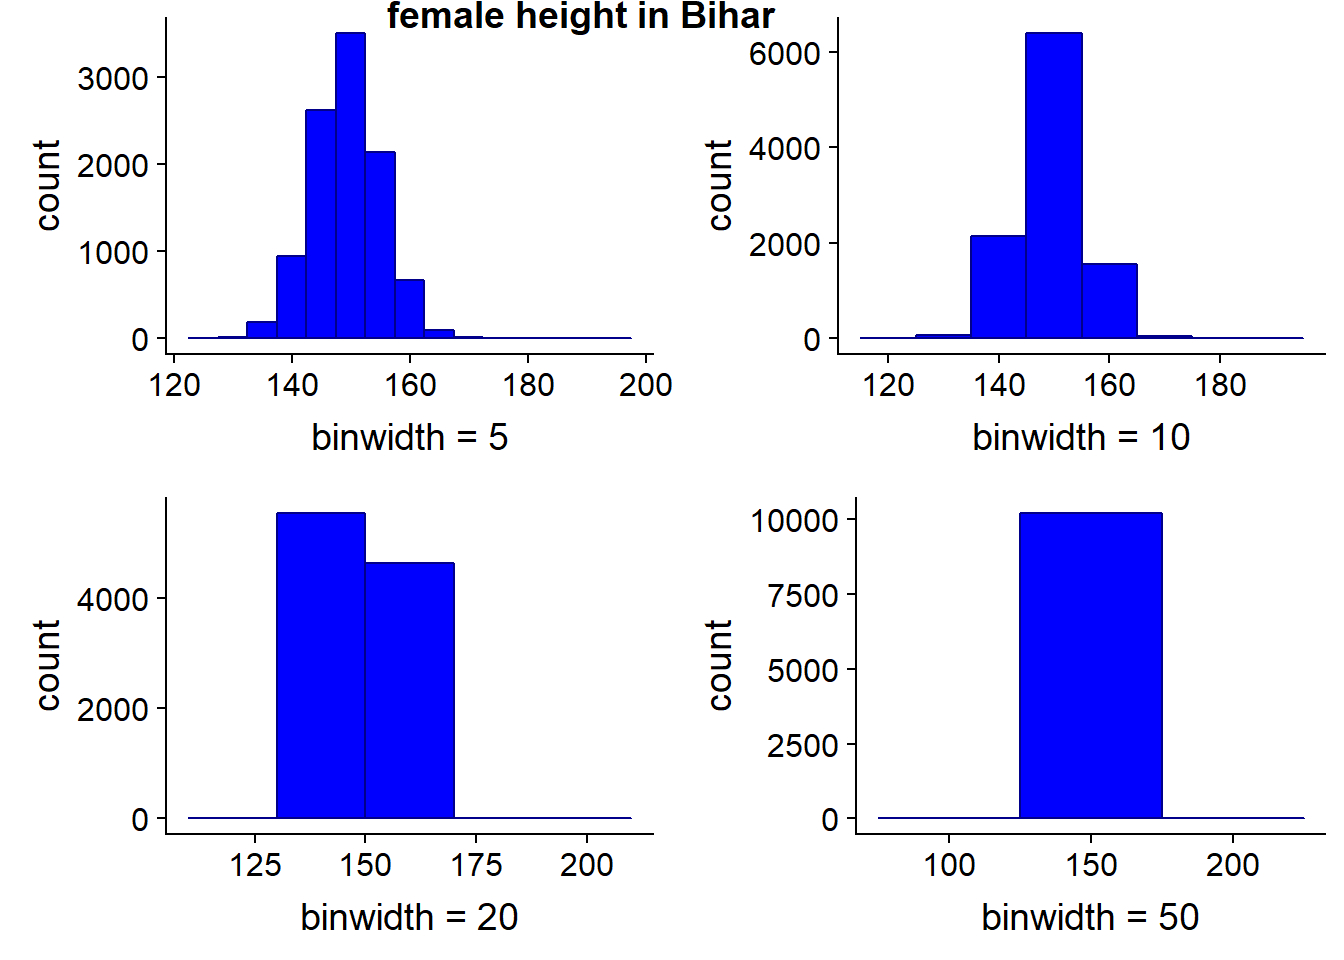
\includegraphics{Module3_files/figure-latex/unnamed-chunk-2-1.pdf}

\begin{Shaded}
\begin{Highlighting}[]
\CommentTok{# we could save the results to an image or a file using }
\CommentTok{# ggsave("folder/bihargrid.pdf")}
\end{Highlighting}
\end{Shaded}

To give a better and smoother representation of the data, we can use a
kernel to visualise the data. It can be thought of as a smoothed
histogram.

\begin{Shaded}
\begin{Highlighting}[]
\KeywordTok{ggplot}\NormalTok{(bihar_adult_females_trunc, }\KeywordTok{aes}\NormalTok{(height_cm)) }\OperatorTok{+}\StringTok{ }
\StringTok{  }\KeywordTok{geom_histogram}\NormalTok{(}\DataTypeTok{data =}\NormalTok{ bihar_adult_females_trunc, }\KeywordTok{aes}\NormalTok{(height_cm, ..density..), }\DataTypeTok{fill =} \StringTok{"white"}\NormalTok{, }\DataTypeTok{color =} \StringTok{"darkred"}\NormalTok{) }\OperatorTok{+}
\StringTok{  }\KeywordTok{geom_density}\NormalTok{(}\DataTypeTok{kernel =} \StringTok{"gaussian"}\NormalTok{, }\KeywordTok{aes}\NormalTok{(height_cm))}
\end{Highlighting}
\end{Shaded}

\begin{verbatim}
## `stat_bin()` using `bins = 30`. Pick better value with `binwidth`.
\end{verbatim}

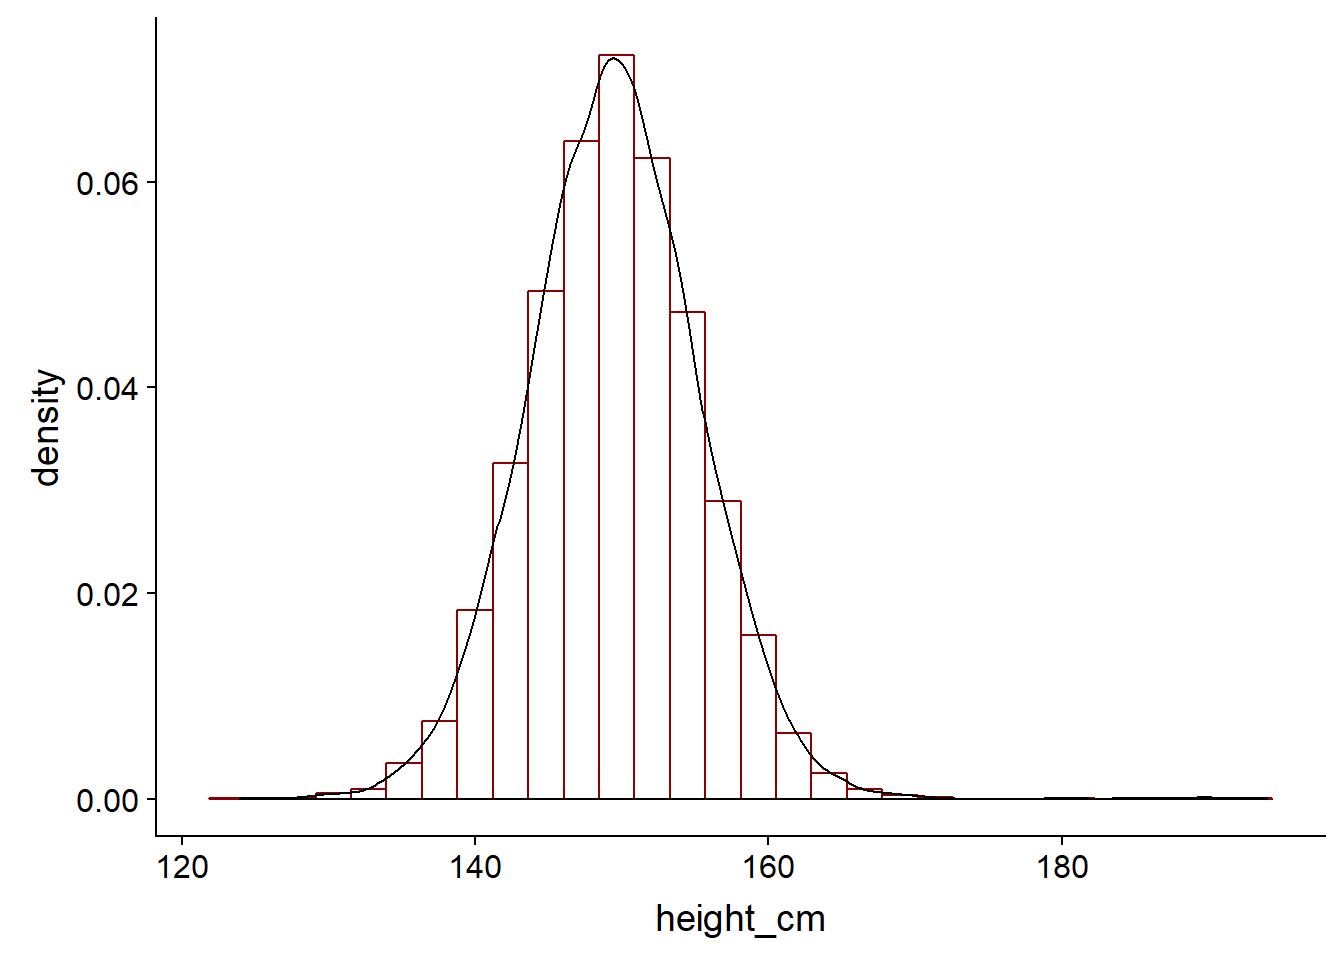
\includegraphics{Module3_files/figure-latex/unnamed-chunk-3-1.pdf}

In practice, it helps us to calculate our probability density function
of the continous variable. As we previously saw, we cannot find the
probability that a particular value of a continous variable is a
particular value - it integrates to zero on a infinitley small scale.
Intead, we can calculate the probability that it takes on some
particular range of values. This is where the Kernel Density Estimation
or KDE comes in.

We can draw a KDE with default parameters - a Gaussian distribution and
auto bin width and no weights - using the density function. The autobin
width are based on Silverman's rule, which the R help notes

\begin{quote}
bw.nrd0 implements a rule-of-thumb for choosing the bandwidth of a
Gaussian kernel density estimator. It defaults to 0.9 times the minimum
of the standard deviation and the interquartile range divided by 1.34
times the sample size to the negative one-fifth power (= Silverman's
`rule of thumb', Silverman (1986, page 48, eqn (3.31))) unless the
quartiles coincide when a positive result will be guaranteed.
\end{quote}

\begin{Shaded}
\begin{Highlighting}[]
\NormalTok{kde =}\StringTok{ }\KeywordTok{density}\NormalTok{(bihar_adult_females_trunc}\OperatorTok{$}\NormalTok{height_cm)}
\KeywordTok{plot}\NormalTok{(kde)}
\end{Highlighting}
\end{Shaded}

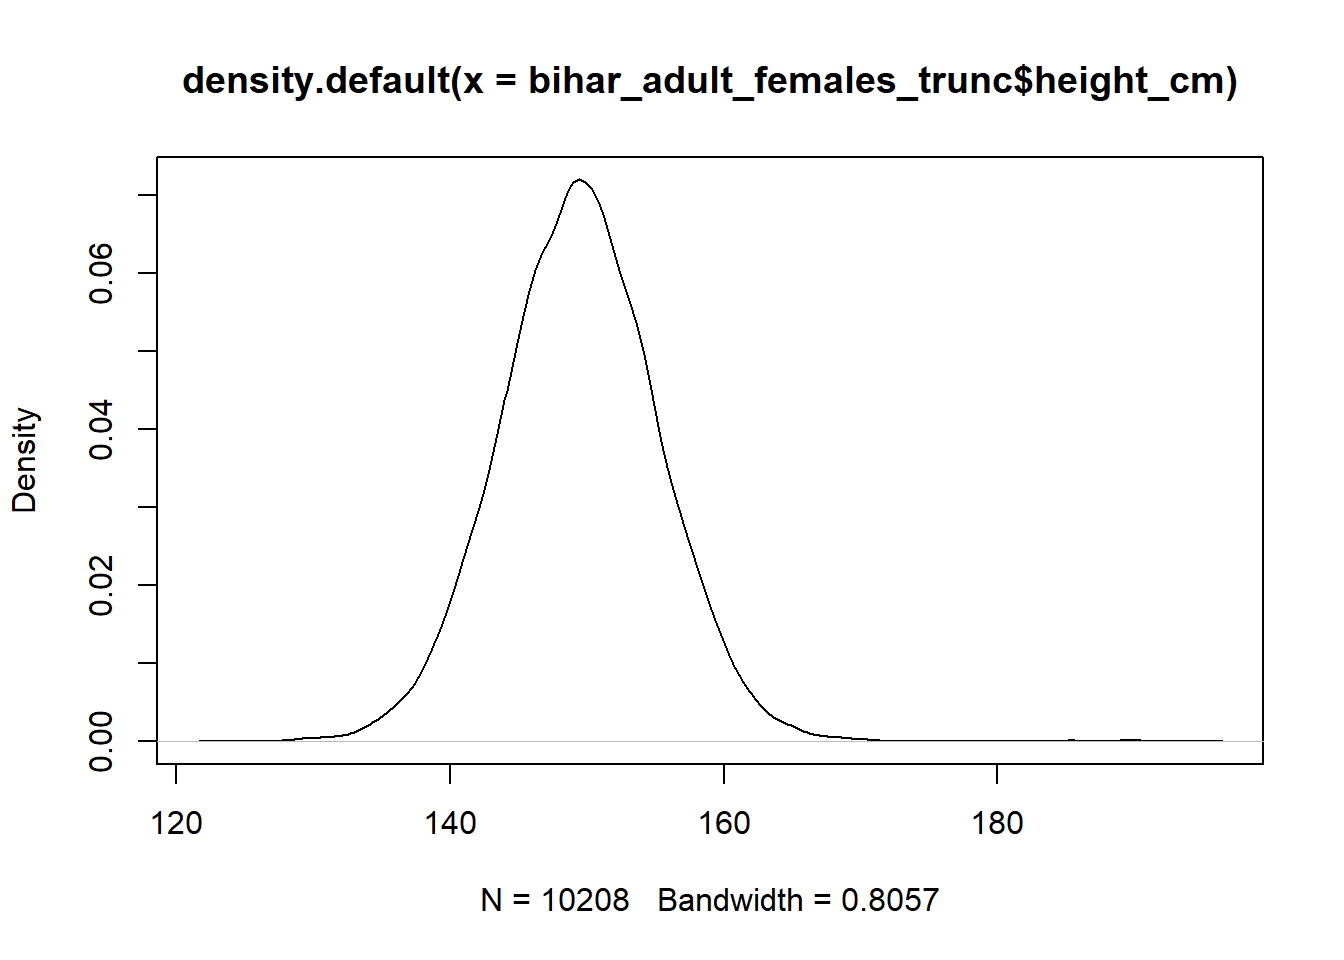
\includegraphics{Module3_files/figure-latex/unnamed-chunk-4-1.pdf}

If we were just calculating a density, then the mathmatical calulcation
would be different than a KDE. KDE is like a weighted distribution,
based on the individual points. A KDE has two paramers, K and h

\begin{itemize}
\tightlist
\item
  K = kernel aka the distribution
\item
  h = smoothing parameter aka bin width
\end{itemize}

There are a number of different kernels, the Guaussian belongs to the
un-bounded which means each event in the study region contributes to the
estimated density at a specific location. This determines the overall
shape of the curve around each of our observations x.

The smoothing parameter helps to determine at each particular point x,
how much other observations around x contribute i.e.~how much they are
weighted. A higher bandwidth will result in a smoother curve, but may
lead to the curve not fitting the underlying data well. The smoothing
parameter also helps to determine the shape, by determining how far
points contribute to the distribution's peak - higher bandwidth results
in points further away having an influence on the PDF and results in a
flatter curve. A lower bandwidth conversely means that only points close
to our particular observation x will play a part i.e.~be weighted, so
will result in a peaked curve around our particular x value.

\[\hat{f} ^{Kernel} (x) = \left. {\frac{1}{Nb} \sum_{i=1}^{N} K (\frac{x - x_i}{b})} \right.\]
* \href{https://www.youtube.com/watch?v=gPWsDh59zdo}{Kernel Density
Estimation video} *
\href{https://en.wikipedia.org/wiki/Kernel_(statistics)}{List of Kernels
in Statistics}

Two of the more common Kernels are the Epanechnikov and Normal
distribution, with the former being bounded (see second link above).

\begin{itemize}
\tightlist
\item
  If the bandwidth is too wide, we will not fit the data well and
  introduce bias, the density plot will look flat and smooth
\item
  If the bandwidth is too narrow, we overfit our data, the density plot
  will look very peaked and jagged
\end{itemize}

The goal is to be somewhere in the middle and to minimise the MSE. MSE
can therefore be thought of as a measure or a quantification of the
amount of the bias/variance tradeoff.

At the extremes, you will introduce some bias, as the kernel will stop
at the boundary of the data, so it will tend to create a peak that is
too high at the point - it it looking at only the data to the right at
the left boundary and vice-versa. It is easier to see this in practice
by looking at plots with higher (wide) bandwidths.

\begin{itemize}
\tightlist
\item
  \href{https://www.youtube.com/watch?v=zrEyxfl2-a8}{Lecture on
  Bias-Variance Tradeoff, from Caltech EdX course}
\end{itemize}

Note - we can either use the stat\_density function or geom\_density -
both are used in the following code as examples. I believe there are
more options with stat\_density.

\begin{Shaded}
\begin{Highlighting}[]
\NormalTok{Bihar5 <-}\StringTok{ }\KeywordTok{ggplot}\NormalTok{(bihar_adult_females_trunc, }\KeywordTok{aes}\NormalTok{(height_cm)) }\OperatorTok{+}\StringTok{ }
\StringTok{  }\KeywordTok{geom_histogram}\NormalTok{(}\DataTypeTok{data =}\NormalTok{ bihar_adult_females_trunc, }\KeywordTok{aes}\NormalTok{(height_cm, ..density..), }\DataTypeTok{fill =} \StringTok{"white"}\NormalTok{, }\DataTypeTok{color =} \StringTok{"darkred"}\NormalTok{) }\OperatorTok{+}
\StringTok{  }\KeywordTok{stat_density}\NormalTok{(}\DataTypeTok{kernel =} \StringTok{"gaussian"}\NormalTok{, }\DataTypeTok{bw =} \DecValTok{1}\NormalTok{, }\KeywordTok{aes}\NormalTok{(height_cm), }\DataTypeTok{fill =} \OtherTok{NA}\NormalTok{, }\DataTypeTok{color =} \StringTok{"darkblue"}\NormalTok{) }\OperatorTok{+}
\StringTok{  }\KeywordTok{xlab}\NormalTok{(}\StringTok{"bandwidth = 1"}\NormalTok{)}

\NormalTok{Bihar6 <-}\StringTok{ }\KeywordTok{ggplot}\NormalTok{(bihar_adult_females_trunc, }\KeywordTok{aes}\NormalTok{(height_cm)) }\OperatorTok{+}\StringTok{ }
\StringTok{  }\KeywordTok{geom_histogram}\NormalTok{(}\DataTypeTok{data =}\NormalTok{ bihar_adult_females_trunc, }\KeywordTok{aes}\NormalTok{(height_cm, ..density..), }\DataTypeTok{fill =} \StringTok{"white"}\NormalTok{, }\DataTypeTok{color =} \StringTok{"darkred"}\NormalTok{) }\OperatorTok{+}
\StringTok{  }\KeywordTok{geom_density}\NormalTok{(}\DataTypeTok{kernel =} \StringTok{"gaussian"}\NormalTok{, }\DataTypeTok{bw =} \DecValTok{5}\NormalTok{, }\KeywordTok{aes}\NormalTok{(height_cm), }\DataTypeTok{fill =} \OtherTok{NA}\NormalTok{, }\DataTypeTok{color =} \StringTok{"darkblue"}\NormalTok{) }\OperatorTok{+}
\StringTok{  }\KeywordTok{xlab}\NormalTok{(}\StringTok{"bandwidth = 5"}\NormalTok{)}

\NormalTok{Bihar7 <-}\StringTok{ }\KeywordTok{ggplot}\NormalTok{(bihar_adult_females_trunc, }\KeywordTok{aes}\NormalTok{(height_cm)) }\OperatorTok{+}\StringTok{ }
\StringTok{  }\KeywordTok{geom_histogram}\NormalTok{(}\DataTypeTok{data =}\NormalTok{ bihar_adult_females_trunc, }\KeywordTok{aes}\NormalTok{(height_cm, ..density..), }\DataTypeTok{fill =} \StringTok{"white"}\NormalTok{, }\DataTypeTok{color =} \StringTok{"darkred"}\NormalTok{) }\OperatorTok{+}
\StringTok{  }\KeywordTok{stat_density}\NormalTok{(}\DataTypeTok{kernel =} \StringTok{"gaussian"}\NormalTok{, }\DataTypeTok{bw =} \DecValTok{10}\NormalTok{, }\KeywordTok{aes}\NormalTok{(height_cm), }\DataTypeTok{fill =} \OtherTok{NA}\NormalTok{, }\DataTypeTok{color =} \StringTok{"darkblue"}\NormalTok{) }\OperatorTok{+}
\StringTok{  }\KeywordTok{xlab}\NormalTok{(}\StringTok{"bandwidth = 10"}\NormalTok{)}

\NormalTok{Bihar8 <-}\StringTok{ }\KeywordTok{ggplot}\NormalTok{(bihar_adult_females_trunc, }\KeywordTok{aes}\NormalTok{(height_cm)) }\OperatorTok{+}\StringTok{ }
\StringTok{  }\KeywordTok{geom_histogram}\NormalTok{(}\DataTypeTok{data =}\NormalTok{ bihar_adult_females_trunc, }\KeywordTok{aes}\NormalTok{(height_cm, ..density..), }\DataTypeTok{fill =} \StringTok{"white"}\NormalTok{, }\DataTypeTok{color =} \StringTok{"darkred"}\NormalTok{) }\OperatorTok{+}
\StringTok{  }\KeywordTok{stat_density}\NormalTok{(}\DataTypeTok{kernel =} \StringTok{"gaussian"}\NormalTok{, }\DataTypeTok{bw =} \DecValTok{20}\NormalTok{, }\KeywordTok{aes}\NormalTok{(height_cm), }\DataTypeTok{fill =} \OtherTok{NA}\NormalTok{, }\DataTypeTok{color =} \StringTok{"darkblue"}\NormalTok{) }\OperatorTok{+}
\StringTok{  }\KeywordTok{xlab}\NormalTok{(}\StringTok{"bandwidth = 20"}\NormalTok{)}

\KeywordTok{plot_grid}\NormalTok{(Bihar5, Bihar6, Bihar7, Bihar8, }\DataTypeTok{labels=}\StringTok{"female height in Bihar"}\NormalTok{, }\DataTypeTok{hjust =} \OperatorTok{-}\DecValTok{1}\NormalTok{, }\DataTypeTok{vjust =} \DecValTok{1}\NormalTok{)}
\end{Highlighting}
\end{Shaded}

\begin{verbatim}
## `stat_bin()` using `bins = 30`. Pick better value with `binwidth`.
## `stat_bin()` using `bins = 30`. Pick better value with `binwidth`.
## `stat_bin()` using `bins = 30`. Pick better value with `binwidth`.
## `stat_bin()` using `bins = 30`. Pick better value with `binwidth`.
\end{verbatim}

\includegraphics{Module3_files/figure-latex/unnamed-chunk-5-1.pdf}

The kernel choice doesn't affect the shape of the curve as much as the
bandwith. The following four charts all have the same bandwidth, but
different kernels. As previously noted, gaussian is unbounded meaning
each point has some weight or contribution to the curve, where as the
others are bounded meaning there is a limit as to which points
contribute i.e.~it has a finite interval. Rectangular and triangular are
the two more unusual shapes compared to the other kernels available.

\begin{Shaded}
\begin{Highlighting}[]
\NormalTok{Bihar9 <-}\StringTok{ }\KeywordTok{ggplot}\NormalTok{(bihar_adult_females_trunc, }\KeywordTok{aes}\NormalTok{(height_cm)) }\OperatorTok{+}\StringTok{ }
\StringTok{  }\KeywordTok{geom_histogram}\NormalTok{(}\DataTypeTok{data =}\NormalTok{ bihar_adult_females_trunc, }\KeywordTok{aes}\NormalTok{(height_cm, ..density..), }\DataTypeTok{fill =} \StringTok{"white"}\NormalTok{, }\DataTypeTok{color =} \StringTok{"darkred"}\NormalTok{) }\OperatorTok{+}
\StringTok{  }\KeywordTok{stat_density}\NormalTok{(}\DataTypeTok{kernel =} \StringTok{"cosine"}\NormalTok{, }\DataTypeTok{bw =} \DecValTok{20}\NormalTok{, }\KeywordTok{aes}\NormalTok{(height_cm), }\DataTypeTok{fill =} \OtherTok{NA}\NormalTok{, }\DataTypeTok{color =} \StringTok{"darkblue"}\NormalTok{) }\OperatorTok{+}
\StringTok{  }\KeywordTok{xlab}\NormalTok{(}\StringTok{"kernel = cosine"}\NormalTok{)}

\NormalTok{Bihar10 <-}\StringTok{ }\KeywordTok{ggplot}\NormalTok{(bihar_adult_females_trunc, }\KeywordTok{aes}\NormalTok{(height_cm)) }\OperatorTok{+}\StringTok{ }
\StringTok{  }\KeywordTok{geom_histogram}\NormalTok{(}\DataTypeTok{data =}\NormalTok{ bihar_adult_females_trunc, }\KeywordTok{aes}\NormalTok{(height_cm, ..density..), }\DataTypeTok{fill =} \StringTok{"white"}\NormalTok{, }\DataTypeTok{color =} \StringTok{"darkred"}\NormalTok{) }\OperatorTok{+}
\StringTok{  }\KeywordTok{stat_density}\NormalTok{(}\DataTypeTok{kernel =} \StringTok{"epanechnikov"}\NormalTok{, }\DataTypeTok{bw =} \DecValTok{20}\NormalTok{, }\KeywordTok{aes}\NormalTok{(height_cm), }\DataTypeTok{fill =} \OtherTok{NA}\NormalTok{, }\DataTypeTok{color =} \StringTok{"darkblue"}\NormalTok{) }\OperatorTok{+}
\StringTok{  }\KeywordTok{xlab}\NormalTok{(}\StringTok{"kernel = epanechnikov"}\NormalTok{)}

\NormalTok{Bihar11 <-}\StringTok{ }\KeywordTok{ggplot}\NormalTok{(bihar_adult_females_trunc, }\KeywordTok{aes}\NormalTok{(height_cm)) }\OperatorTok{+}\StringTok{ }
\StringTok{  }\KeywordTok{geom_histogram}\NormalTok{(}\DataTypeTok{data =}\NormalTok{ bihar_adult_females_trunc, }\KeywordTok{aes}\NormalTok{(height_cm, ..density..), }\DataTypeTok{fill =} \StringTok{"white"}\NormalTok{, }\DataTypeTok{color =} \StringTok{"darkred"}\NormalTok{) }\OperatorTok{+}
\StringTok{  }\KeywordTok{stat_density}\NormalTok{(}\DataTypeTok{kernel =} \StringTok{"rectangular"}\NormalTok{, }\DataTypeTok{bw =} \DecValTok{20}\NormalTok{, }\KeywordTok{aes}\NormalTok{(height_cm), }\DataTypeTok{fill =} \OtherTok{NA}\NormalTok{, }\DataTypeTok{color =} \StringTok{"darkblue"}\NormalTok{) }\OperatorTok{+}
\StringTok{  }\KeywordTok{xlab}\NormalTok{(}\StringTok{"kernel = rectangular"}\NormalTok{)}

\NormalTok{Bihar12 <-}\StringTok{ }\KeywordTok{ggplot}\NormalTok{(bihar_adult_females_trunc, }\KeywordTok{aes}\NormalTok{(height_cm)) }\OperatorTok{+}\StringTok{ }
\StringTok{  }\KeywordTok{geom_histogram}\NormalTok{(}\DataTypeTok{data =}\NormalTok{ bihar_adult_females_trunc, }\KeywordTok{aes}\NormalTok{(height_cm, ..density..), }\DataTypeTok{fill =} \StringTok{"white"}\NormalTok{, }\DataTypeTok{color =} \StringTok{"darkred"}\NormalTok{) }\OperatorTok{+}
\StringTok{  }\KeywordTok{stat_density}\NormalTok{(}\DataTypeTok{kernel =} \StringTok{"triangular"}\NormalTok{, }\DataTypeTok{bw =} \DecValTok{20}\NormalTok{, }\KeywordTok{aes}\NormalTok{(height_cm), }\DataTypeTok{fill =} \OtherTok{NA}\NormalTok{, }\DataTypeTok{color =} \StringTok{"darkblue"}\NormalTok{) }\OperatorTok{+}
\StringTok{  }\KeywordTok{xlab}\NormalTok{(}\StringTok{"kernel = triangular"}\NormalTok{)}

\KeywordTok{plot_grid}\NormalTok{(Bihar9, Bihar10, Bihar11, Bihar12, }\DataTypeTok{labels=}\StringTok{"Bandwidth 20, varying kernel"}\NormalTok{, }\DataTypeTok{hjust =} \OperatorTok{-}\DecValTok{1}\NormalTok{, }\DataTypeTok{vjust =} \DecValTok{1}\NormalTok{)}
\end{Highlighting}
\end{Shaded}

\begin{verbatim}
## `stat_bin()` using `bins = 30`. Pick better value with `binwidth`.
## `stat_bin()` using `bins = 30`. Pick better value with `binwidth`.
## `stat_bin()` using `bins = 30`. Pick better value with `binwidth`.
## `stat_bin()` using `bins = 30`. Pick better value with `binwidth`.
\end{verbatim}

\includegraphics{Module3_files/figure-latex/unnamed-chunk-6-1.pdf}

\bibliography{book.bib}


\end{document}
